\documentclass[oneside]{mgr}

\usepackage{polski}      
\usepackage[utf8]{inputenc}
\usepackage[T1]{fontenc} 
\usepackage{indentfirst}
\usepackage{textcomp}
\usepackage{gensymb}
\usepackage{color}
\usepackage[table]{xcolor}
\usepackage{multirow}
\usepackage{multicol}
\usepackage{ltablex}
\usepackage{caption}


%pakiety do grafiki
\usepackage{graphicx}
\usepackage{subfigure}
\usepackage{psfrag}


\usepackage{amsmath}
\usepackage{amsfonts}

\usepackage{supertabular}
\usepackage{array}
\usepackage{tabularx}
\usepackage{hhline}
\usepackage{showlabels}
\usepackage{gensymb}

%definicje własnych poleceń
\newcommand{\R}{I\!\!R} %symbol liczb rzeczywistych, działa tylko w
                        %trybie matematycznym
\newtheorem{theorem}{Twierdzenie}[section] %nowe otoczenie do
                                           %składania twierdzeń
\title{Badanie pracy wentylatorowego układu chłodzenia z ogniwami Peltiera}
\engtitle{Control of the cooling system with Peltier module}
\author{Piotr Bogaczyk}
\supervisor{dr inż. Jacek Jagodziński W-4/K-8}
\field{Automatyka i Robotyka (AIR)}
\specialisation{Systemy informatyczne w automatyce (ASI)}

\begin{document}
\maketitle
\tableofcontents

\chapter{Wstęp}

Ogniwo Peltiera to element termoelektryczny, który w zależności od kierunku przepływu prądu pochłaniania lub wydziela energię cieplną na przeciwległych stronach ogniwa. Wykonany jest z wielu połączonych szeregowo i naprzemiennie półprzewodników typu „p” i „n”, umieszczonych pomiędzy dwoma cienkimi płytkami ceramicznymi. Oprócz chłodzenia i ogrzewania ogniwo Peltiera może też być wykorzystane do wytwarzania energii elektrycznej. Energia ta powstaje w wyniku zjawiska Seebecka, gdy pod wpływem różnicy temperatur po obu stronach modułu generowana jest siła elektromotoryczna.
Ogniwa Peltiera dzięki prostej budowie, braku części ruchomych oraz czynnika chłodzącego odznaczają się dużą trwałością. Małe wymiary i łatwa regulacja mocy skłania do ich coraz powszechniejszego zastosowania w wielu dziedzinach życia: od urządzeń domowych poprzez sprzęt medyczny i wojskowy aż po technologie kosmiczne.

Tematem niniejszej pracy jest projekt układu dla badania ogniwa Peltiera oraz wykorzystanie wykonanych badań w celu usprawnienia regulacji temperatury w komorze chłodniczej. Praca składa się z pięciu głównych części. Pierwsza z nich opisuje podstawowe prawa i zasady termoelektryczne takie jak efekt Seebecka, efekt Peltiera oraz efekt Thomsona. Druga zawiera opis realizacji urządzenia badawczego w skład rozdziału wchodzi opis układu chłodniczego z wykorzystaniem ogniwa Peltiera oraz opis wszystkich elementów wykorzystanych w projekcie. Trzecia część zawiera opis wykorzystanych programów komputerowych oraz oprogramowania wykorzystywanego do zbierania danych pomiarowych z obiektu badawczego jak i opis programu wykorzystanego do programowania sterownika PLC wykorzystanego w projekcie. Czwarta część zawiera opis wykonanych badań pozwalających na obliczenie maksymalnej mocy chłodniczej ogniwa wraz z jego sprawnością w zależności od podawanego na ogniwo natężenia i napięcia prądu elektrycznego. Piąta część opisuje porównanie zastosowanych sposobów regulacji temperatury wewnątrz komory termicznej z wykorzystaniem ogniwa Peltiera. Dodatkowo w pracy zostały zawarte schematy elektryczne wykorzystanych urządzeń elektrycznych wykonane przy pomocy programu Eplan.

\section{Cel i zakres pracy}

Celem pracy jest zaprojektowanie, budowa i wysterowanie komory termicznej wykorzystującej ogniwo Peltiera jako pompę ciepła.

W pracy została opisana zasada działania oraz budowa modułu Peltiera. Opisano również podstawowe zjawiska termoelektryczne które towarzyszą zmianą temperatury w badanych ogniwach termoelektrycznych.

Został zbudowany obiekt badawczy pozwalający na grzanie lub chłodzenie przestrzeni wewnątrz kasety wykonanej z szkła akrylowego. Efekty działania urządzenia badane są przy wykorzystaniu trzech czujników temperatury typu PT0-10. Czujniki pozwalają one na pomiar temperatury ciepłej i chłodnej strony ogniwa Peltiera oraz pomiar temperatury bezpośrednio wewnątrz zbudowanej komory termicznej. Transmisja ciepła pomiędzy otoczeniem a modułem Peltiera zostało usprawnione przez wykorzystane w projekcie radiatory wspomagane wentylatorami. Dodatkowo wewnątrz komory zostały zamontowane cztery rezystory wysokich mocy. Rezystory zostały zastosowane w celu wprowadzania do układu zakłóceń.

W celu badania, regulacji i wysterowania zbudowanego układu zastosowany został sterownik serii: LOGO!8 marki Siemens. Sterownik pozwala na płynną regulację temperatury wewnątrz komory termicznej. Regulacji temperatury dokonuje się na podstawie odczytu danych z trzech czujników temperatury wykorzystanych w projekcie. W pracy zostały przedstawione i przeanalizowane trzy typy regulacji: krokowa, typu PI oraz predykcyjna.

\section{Założenia projektowe}
Praca zakłada stworzenie układu pozwalającego na płynną regulację temperatury w komorze termicznej z wykorzystaniem sterownika LOGO!8. W pracy założono ,że temperatura na zewnątrz stacji jest stała i niezmienna w czasie.

Sygnały pomiarowe oraz sterujące są przekazywane do i z sterownika za pomocą przewodów poprowadzonych w zamaskowanych szynach. Projekt zakłada brak zakłóceń transmisji sygnałów.

Praca zawiera schematy elektryczne które zostały wykonane za pomocą programu EPLAN w standardzie jednokreskowym. Wszystkie schematy zostały wykonane zgodnie z praktyką inżynierską i zawarte w załączniku numer 1: „Schematy elektryczne”.

\chapter{Teoria chłodnictwa termoelektrycznego}
Istotą modułów Peltiera są zmiany temperatury które zachodzą na złączach półprzewodnikowych (n-p lub p-n) pod wpływem przepływu przez nie prądu elektrycznego. Takie zmiany temperatury znajdują szerokie zastosowanie w chłodnictwie. Zastosowanie ogniw Peltiera w chłodnictwie pozwala na wysoce bezawaryjną pracę chłodziarki w różnych orientacjach. 
Ponieważ napięcie elektryczne jest łatwe do kontrolowania i może być dokładnie zmierzone, urządzenia wykorzystujące efekt termoelektryczny umożliwiają bardzo precyzyjną regulację temperatury i automatyzację procesów chłodzenia i ogrzewania. W zależności od kierunku transformacji efekty termoelektryczne dzielą się na: efekt Seebecka, Peltiera i Thomsona.

\section{Efekt Seebecka}
Efekt Seebecka polega na powstawaniu siły termoelektrycznej w otwartym obwodzie złożonym z dwóch różnych półprzewodników jeżeli ich spoiny są utrzymywane w różnych temperaturach. Przy zamknięciu obwodu następuje przepływ prądu który ściśle zależy od różnicy temperatur półprzewodników oraz materiałów z których są wykonane. Obwód taki nazywany jest termoelementem w technice chłodniczej oraz termoparą w technice cieplnej[1].
\begin{eqnarray}
    e_{AB}(T) \approx U_0 + \alpha \cdot T\\
    e_{BA}(T) \approx -U_0 -\alpha \cdot T_0 \nonumber
\end{eqnarray}
gdzie: \\
$U_0$ napięcie kontaktowe \\
$T$,$T_0$ – temperatura złączy materiałów $A$ i $B$ \\
$\alpha$ - współczynnik Seebecka obwodu \\

W przewodnikach typu "p-n" występują dwa typy przewodności. Odpowiednio przewodność elektronowa w której nośnikami ładunków są elektrony i dziurowa w której nośnikami są dodatnio naładowane dziury. Jeśli moduł składa się z półprzewodników tego samego typu, w takim wypadku siły termoelektryczne które występują w obwodzie posiadają przeciwne zwroty[1]:
\begin{eqnarray}
    a_p=a_{p1}-a_{p2}, \qquad a_n=a_{n1}-a_{n2}
\end{eqnarray}
Przy różnych rodzajach przewodności spoin siły termoelektromotoryczne sumują się:
\begin{eqnarray}
    \Bar{\alpha}=|\alpha_p|+|\alpha_n|
\end{eqnarray}

W konsekwencji termoelementy wykonuje się głównie z materiałów o różnej przewodności: elektronowej i dziurowej. Każdy zestaw p-n składa się z dwóch gałęzi: typu "n" oraz "p" nazywanych również półelementami. Półelementy typu "p" oraz "n" są połączone ze sobą tak zwanymi mostkami do których są przymocowane przy pomocy lutowania miękiego lub specjalistycznego kleju przewodzącego. Mostki łączące zwykle wykonuje się z miedzi[1] (rys. 2.1)

Takie szeregowe naprzemienne połączenie par przewodników "p" i "n" stanowi siłę termoelektromotoryczną modułu. Wyznacza się ją z zależności[1]:

\begin{eqnarray}
    E = n \int_{T_{gor}}^{T_z}(|\alpha_p|+|\alpha_n|)dT
\end{eqnarray}
gdzie: \\
$n$ - liczba termoelementów, \\
$T_{gor}$ - temperatura strony gorącej termoelementu, \\
$T_z$ - temperatura strony zimnej termoelementu.
\section{Efekt Peltiera}
Efektem Peltiera nazywamy zjawisko odwrotne do zjawiska Seebecka, polega ono na wydzielaniu się lub pochłanianiu ciepła na spoinach termoelementu w trakcie przepływu przez niego prądu. Strumień takiego ciepła nazywany jest ciepłem Peltiera i można go wyznaczyć przy pomocy wzoru[1]:
\begin{equation}
    Q_p = \pi I
\end{equation}
gdzie: \\
$\pi$ - współczynnik Peltiera, \\
$I$ - natężenie prądu. \\

W zależności od kierunku przepływu prądu ciepło może być pochłaniane lub oddawane do otoczenia.
\section{Efekt Thomsona}
Chronologicznie trzecim odkrytym efektem termoelektrycznym jest efekt Thomsona. Jego istotą jest to, że przy przepływie prądu stałego przez przewodnik lub półprzewodnik, w którym już istnieje gradient temperatury, w uzupełnieniu do ciepła Joule'a wydziela się, bądź jest pochłaniana pewna ilość ciepła które nazywane jest ciepłem Thomsona[1]. Jest to spowodowane zwiększaniem się energii elektronów swobodnych wraz z wzrostem temperatury. Dla metali wykorzystywanych w termoelementach efekt Thomsona jest minimalny i można go nie uwzględniać w obliczeniach.

W trakcie pracy termoelementu można zaobserwować wszystkie trzy zjawiska: Seebecka, Peltiera oraz Thomsona które wzajemnie na siebie oddziałują.

Jedną z zależności jest zależność współczynnika Peltiera od siły termoelektromotorycznej:
\begin{equation}
    \pi = \alpha T
\end{equation}
Również można zauważyć zależność współczynnikami siły termoeletromotorycznej a współczynnikiem Thomsona $\beta$:
\begin{equation}
    \beta = (\frac{d\alpha}{dt})T
\end{equation}

Powyższe równanie przedstawia zależność współczynnika $\beta$ od znaku pochodnej $\frac{d\alpha}{dt}$. Generalnie stosunek siły termoelektrycznej do temperatury ma charakterystykę nieliniową z przedziałami zarówno rosnącymi jak i malejącymi. Zatem dla jednego materiału współczynnik Thomsona może być zarówno ujemny jak i dodatni.

\section{Termoelektryczny moduł Peltiera}
\subsection{Budowa i działanie modułów termoelektrycznych:}
Ogniwo Peltiera nazywane również modułem Peltiera bądź płytką Peltiera jest półprzewodnikowym elementem termoelektrycznym, który wykorzystuje zjawisko Peltiera do wymiany ciepła. Typowy moduł składa się z dwóch równolegle ułożonych do siebie płytek ceramicznych pomiędzy którymi na przemian są rozmieszczone półprzewodniki typu "n" oraz "p". Naprzemiennie ułożone półprzewodniki wykonane są z odpowiednio domieszkowanego tellurku bizmutu i są one ze sobą połączone szeregowo przy pomocy miedzianych płytek.

\begin{figure}[h]
    \centering
    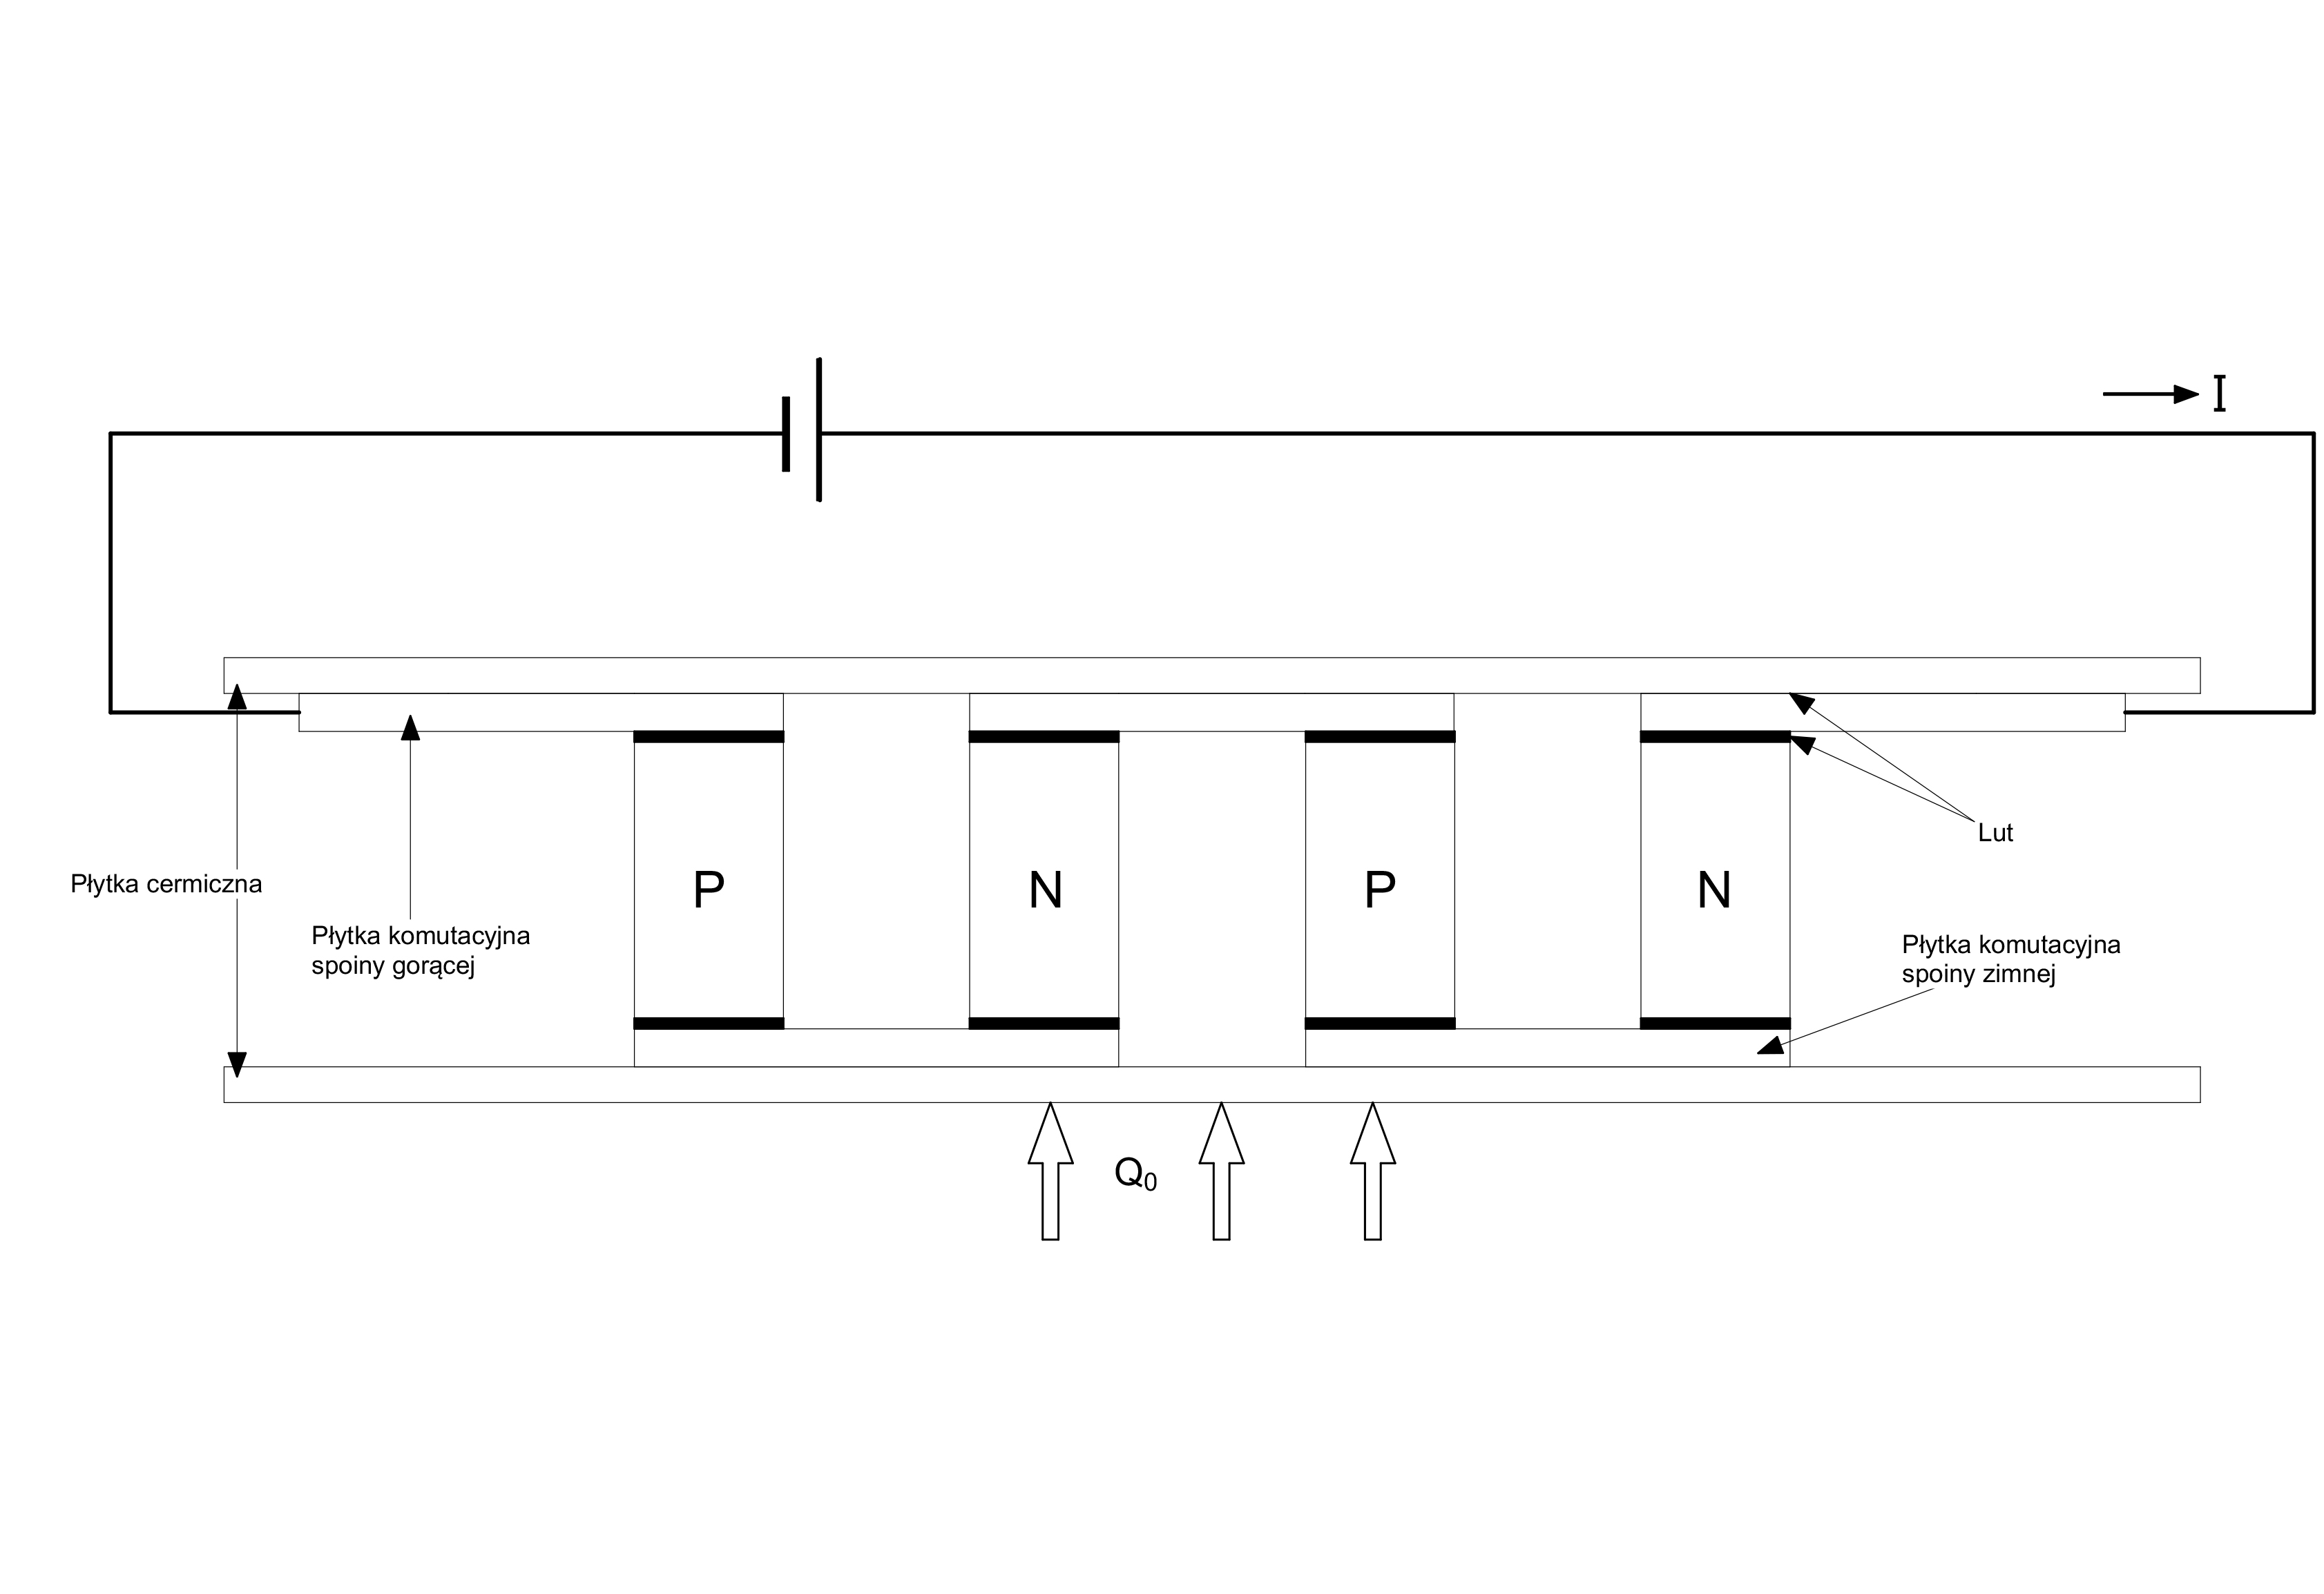
\includegraphics[width=\textwidth]{modul_peltiera.jpg}
    \caption{Schemat ideowy modułu Peltiera}
\end{figure}

Półprzewodnik typu „p” nie ma w swojej strukturze wystarczającej ilości elektronów, aby całkowicie „wypełnić” górny poziom energetyczny, podczas gdy półprzewodnik typu „n” ma ich zbyt wiele. W momencie zasilenia modułu prądem elektrycznym elektrony poruszają się między poziomami energii - co w jednym przypadku wymaga energii (przejście na wyższy poziom energetyczny), a w innym powoduje jej emisję (spadek do niższego poziomu) - w zależności od kierunku przepływu prądu. Zarówno zużyta energia, jak i oddana są w tym przypadku energią cieplną. Na górnej jak i dolnej powierzchni jednocześnie zachodzi pochłanianie ciepła („zimna strona”) i jego oddawanie („gorąca strona”). Dlatego działanie modułów termoelektrycznych często jest porównywane do działania pompy cieplnej.

Ilość ciepła, które można transportować w ten sposób, zależy od natężenia przyłożonego do termoelementu prądu elektrycznego. Można zaobserwować fakt, że gdy prąd przepływa przez system, pewna ilość ciepła powstaje również w samym module (z powodu rezystancji elektrycznej powstaje ciepło Joule'a). Z tego powodu każdy moduł Peltiera charakteryzuje się  pewną maksymalną wydajnością cieplną.

Ważną cechą jest również możliwość łączenia modułów tak, aby „zimna” strona następnego modułu przylegała do „gorącej” strony poprzedniego modułu,
co skutkuje uzyskaniem wyższej wydajności. Biorąc pod uwagę ciepło wytwarzane przez rezystancję prądu elektrycznego, który jest również odprowadzany do „gorącej” strony, takie połączenia są zwykle wykonywane w sposób piramidalny - tak że końcowa powierzchnia emitująca ciepło jest większa niż powierzchnia pochłaniająca. Takie połączenie modułów termoelektrycznych, pod względem zwiększenia wydajności stanowi alternatywę dla zwiększenia prądu przepływającego przez system.

Z uwagi na dużą ilość energii cieplnej(od kilkunastu do nawet kilkuset wat) oddawanej przez "gorącą" stronę, zaleca się stosowanie dodatkowego chłodzenia do ogniw. Najczęściej wykorzystuje się w tym celu radiatory które mogą być dodatkowo wentylowane. Ważne jest również użycie pomiędzy ogniwem a elementem odprowadzającym ciepło pasty przewodzącej która poprawia przepływ ciepła. Wykorzystanie dodatkowych form odprowadzania ciepła ma szczególne znaczenie w przypadku łączenia termoelementów kiedy energia cieplna emitowana przez nie kumuluje się na każdym kolejnym poziomie. 

\subsection{Parametry modułów termoelektrycznych}

W większości literatury parametry ogniw termoelektrycznych są dzielone na dwie grupy: użytkowe i konstrukcyjne. Jednym z głównych parametrów ogniw jest ich maksymalna wydajność chłodnicza $Q_{0(\max)} [W]$ i wytwarzana maksymalna różnica temperatur pomiędzy zimną a ciepłą stroną ogniwa $\Delta T_{\max} [^{\circ} C]$

$Q_{0(\max)}$ wyznaczane jest przy stałej temperaturze górnego źródła ciepłą(z zasady $T_{gor}=+27^\circ C$)[1] i przy zerowej różnicy temperatur pomiędzy stroną zimną a ciepłą modułu czyli $\Delta T_{\max} = T_{gor} - T_z = 0 [^{\circ} C]$. $\Delta T_{\max}$ wyznaczane jest gdy ogniwo nie jest cieplnie obciążone, wtedy gdy wartość $Q_0 = 0$ i gdy temperatura strony gorącej jest stała.

Przedstawione dwie podstawowe wartości odpowiadają punktom przecięcia $Q_0 (\Delta T)$ z osiami układów współrzędnych[1]. Ważną wielkością umieszczaną w charakterystyce każdego modułu jest również $I_{opt}$ jak i inne ważne parametry eksploatacyjne takie jak np. napięcie zasilania czy opór elektryczny modułu.

Oporem prądu zmiennego jest nazywana rezystancja występująca przy $\Delta T = 0$ a więc przy zerowej różnicy temperatur pomiędzy stroną gorącą a zimną ogniwa. Przyjęło się ,że opór taki przyjmuje oznaczenie $R_\sim$, opór prądu stałego jest oznaczany natomiast symbolem $R_=$. Z powodu działania elektrodynamicznej siły Seebecka opór elektryczny termoelementu znacząco zmniejsza się wraz z wzrostem temperatury spoin. Dlatego rozróżniane są różne rezystancje. Opisane wartości opisuje zależność:
\begin{equation}
    U = IR_ = (\text{przy założeniu } \Delta T = \text{const})
\end{equation}

Z kolei parametry konstrukcyjne modułów termoelektrycznych to między innymi:
\begin{itemize}
    \item wymiary modułu (wysokość, szerokość i długość podawana w milimetrach),
    \item masa modułu (podawana w gramach),
    \item materiał z którego ogniwo zostało wykonane,
    \item ilość naprzemiennie ułożonych złącz p-n,
    \item przewidywany czas pracy lub średni okres lat działania,
    \item maksymalna ilość przełączeń trybów pracy (grzanie/chłodzenie).
\end{itemize}

\subsubsection{Parametr Z modułu i jego pomiar}
Z przytoczonych wyżej informacji wynika, że materiał z którego wykonane są złącza p-n powinien mieć jak najmniejszą rezystancję i przewodność cieplną a jak najlepsze właściwości związane z zjawiskiem Peltiera. Niestety obie te wymagania wzajemnie się wykluczają.

W celu uzyskania jak najmniejszego oporu modułu termoelektrycznego jego złącza powinny mieć jak największy przekrój i być jak najniższe, jednakże takie rozwiązanie spowoduje szybkie nagrzewanie się strony zimnej od strony gorącej. Dlatego konstrukcja modułu termoelektrycznego wymaga znalezienia złotego środka pomiędzy opornością a wysokością złącz.

W celu wyznaczenia dobroci materiału i jego przydatności do budowy ogniw Peltiera wprowadzono parametr $Z$ którego pomiaru dokonuje się metodą Harmana:
\begin{equation}
    Z = \frac{\alpha^2}{kR}
\end{equation}
gdzie: \\
$k$ - współczynnik przenikania ciepła, \\
$R$ - wartość oporu elektrycznego, \\
$\alpha$ - średnia wartość współczynnika siły termoelektromotorycznej dwóch gałęzi w przedziale temperatur $T_{gor}-T_z$. \\

Z dotychczasowo znanej literatury wynika[1], że najlepszą dobrocią charakteryzuje się wcześniej wspomniany półprzewodnik tellurek bizmutu - $Bi_2 Te_3$.

\subsubsection{Pomiar i wyznaczenie maksymalnej różnicy temperatur $\Delta T_{\max}$}

Pomiaru maksymalnej różnicy temperatur strony zimnej i gorącej modułu termoelektrycznego dokonuje się za pomocą systemu składającego się z bardzo dobrze chłodzonej podstawy. Chłodzenie najczęściej jest realizowane przy pomocy radiatora dodatkowo chłodzonego wodą bądź powietrzem której temperatura jest utrzymywana na stałym poziomie. Do połączenia modułu z radiatorem stosuje się pastę termoprzewodzącej która poprawia przewodnictwo cieplne układu. Bezpośrednio przy stronie zimnej jak i gorącej modułu w odpowiednich zagłębieniach znajdują się czujniki temperatury które mierzą $T_{gor}$ oraz $T_{ch}$ modułu. W przestrzeni w której znajduje się badany obiekt w celu zmniejszenia obciążenia cieplnego stosuje się obniżenie ciśnienia do $10^{-3} \dots 10^{-4}$ mmHg. Dalsze obniżanie ciśnienia nie ma wpływu na polepszenie dokładności wyników pomiarów. W celu dalszej poprawy wyników stosuje się ograniczenie dostępności światła do obiektu bądź otoczenie całego systemu odpowiednim ekranem chłodzącym którego temperatura będzie utrzymywany blisko $T_{ch}$. Poprzez stopniowe zwiększanie natężenia prądu można wyznaczyć minimalną temperaturę strony zimnej. Pozwala to na obliczenie $\Delta T_{\max}$ i parametru $Z$. Wykorzystanie tej metody do wiliczenia parametru $Z$ nie uwzględnia ciepła Thomsona[1], co powoduje zawyżenie wartości $Z$.

Na podstawie[1] w celu dokładnego wyznaczenia parametru $Z$ należy skorzystać z poprawionego wzoru:
\begin{equation}
    Z = 2 \Delta T_{\max}/{T_{ch}^2}_{(\min)}[1/3(\Delta T_{\max}/T_{ch}(\beta/\alpha))]
\end{equation}
gdzie:\\
$\beta$ - współczynnik Thomsona z równania (2.7). \\

A więc aby precyzyjniej wyznaczyć parametr $Z$ należy znać $\alpha$ oraz $\beta$. Aby uzyskać jak najbardziej dokładne wyniki należy zadbać aby chłodzenie badanego modułu było jak najlepsze poprzez chłodzenie powietrzem bądź wodą. Zabieg taki pozwoli na ograniczenie podgrzewania strony grzejącej ogniwa przez stronę chłodzącą.

Zmierzone $\Delta T_{\max}$ przedstawioną powyżej metodą(pomiar dokonywany w próżni) z reguły można znaleźć w kartach katalogowych modułów termoelektrycznych. Te same badania wykonane bez wykorzystania próżni pozwala na uzyskanie wyników około 20\% mniejszych.

\subsubsection{Wyznaczenie i pomiar $Q_{0(\max)}$ modułu}

Stanowisko do pomiaru parametru $Q_{0(\max)}$ modułu termoelektrycznego wygląda podobnie do stanowiska do pomiaru $\Delta T_{\max}$ z tą różnicą ,że zamiast stosowania próżni stosuje się odpowiednią izolację termiczną. Zabieg ten wykonuje się w celu ograniczenia wpływu ciepła pochodzącego z otoczenia na badany moduł. Najczęściej wykorzystywanym materiałem do izolacji obiektu jest poliuretan o grubości do 50 mm. Moduł termoelektryczny zasilany jest przy pomocy zasilacza, pozwalającego w precyzyjny sposób kontrolować napięcie i natężenie prądu elektrycznego. Wymnożenie napięcia i natężenia prądu pozwala otrzymać moc elektryczną. Przyjmuje się ,że 100\% tej mocy zamienia się na ciepło ,które przejmuje moduł[1]. Zastosowane termoelektryczne czujniki temperatury bezpośrednio przy stronie chłodnej i gorącej modułu pozwalają na bieżący pomiar temperatury. Poprzez równomierne zwiększanie napięcia, należy ustalić stan równowagi w którym $\Delta T = 0$ a więc temperatura strony gorącej modułu zrówna się z temperaturą strony chłodnej. Uzyskana w taki sposób moc jest maksymalną wydajnością chłodniczą modułu termoelektrycznego $Q_{0(\max)}$. Ważne jest aby wszystkie parametry wyznaczać przy zbliżonych warunkach początkowych.

\subsection{Wykorzystanie ogniw Peltiera}

Ogniwa Peltiera dzięki swojej nieskomplikowanej budowie, małym rozmiarom oraz niezawodności znalazły szerokie zastosowanie jako pompy cieplne. Ogniwa stosuje się do budowy urządzeń chłodniczych wykorzystywanych w sprzętach gospodarstwa domowego jak i w zaawansowanych technologicznie systemach chłodzenia wykorzystywanych w przemyśle oraz medycynie. Stanowią one doskonałe uzupełnienie sprzętu chłodniczego gdy zależy nam na pracy układu w różnych położeniach jak i braku szkodliwych substancji (np. freonu).

Najczęściej moduły Peltiera stosuje się:
\begin{itemize}
    \item chłodzenie nagrzewających się urządzeń elektrycznych
    \item komory klimatyczne
    \item chłodzenie diod wykorzystywanych w laserach wysokich mocy
    \item przenośne i stacjonarne urządzenia klimatyzacyjne
    \item termostaty wykorzystywane w akwarystyce
    \item przenośne lodówki
\end{itemize}

Niezwykle ważnym zastosowaniem ogniw Peltiera jest również wykorzystywanie ich do produkcji prądu elektrycznego korzystając z zjawiska Seebecka. Ciekawostką jest fakt, że niektóre bezzałogowe statki kosmiczne (w tym łazik Curiosity Mars) wykorzystują radioizotopowe generatory termoelektryczne (RTG), które przekształcają energię cieplną w energię elektryczną za pomocą efektu Seebecka. Urządzenia mogą przetrwać kilka dziesięcioleci, ponieważ ich zasilanie odbywa się przez rozpad wysokoenergetycznych materiałów radioaktywnych.[16]

\chapter{Realizacja stacji badawczej z komorą termiczną}
\section{Opis obiektu}

W celu zrealizowania układu pozwalającego na badanie i regulacje temperatury z wykorzystaniem ogniw Peltiera został zbudowany obiekt badawczy. Urządzenie składa się z stelażu wykonanego z profili aluminiowych na którym zostały osadzone urządzenia sterujące, pomiarowe oraz wykonawcze. Dodatkowo została wykonana zamknięta komora badawcza ze szkła akrylowego o grubości 6$mm$ która ogranicza emisję ciepła do otoczenia. Istnieje możliwość wyjęcia całego systemu chłodzącego w skład którego wchodzi ogniwo wraz z radiatorami i wentylatorami. Aby tego dokonać należy odłączyć złącze, odkręcić śrubki motylkowe i delikatnie wysunąć górną część komory wraz z wszystkimi elementami wykonawczymi. Zabieg ten może zostać wykonany w wypadku konieczności konserwacji urządzenia, wyczyszczenia komory chłodzącej bądź też wymiany ogniwa Peltiera. 

Temperatura wewnątrz komory badawczej może być zakłócana poprzez zastosowanie czterech sterowanych analogowo rezystorów wysokich mocy. Każdy z rezystorów charakteryzuje się mocą 50W. Urządzenie pozwala na regulację mocą grzewczą rezystorów w zakresie 0-100\%. Zasilanie wszystkich urządzeń realizowane jest przy pomocy zasilacza 24 V.

Elementami pomiarowymi które są odpowiedzialne za mierzenie temperatury  w czasie rzeczywistym są trzy czujniki temperatury ($T_1, T_2, T_3$) które zostały zainstalowane bezpośrednio przy stronie gorącej oraz zimnej modułu jak i wewnątrz komory termicznej. Takie rozwiązanie pozwala na zmierzenie różnicy temperatur po stronie gorącej i chłodnej ogniwa oraz wewnątrz zbudowanej komory termicznej. Dodatkowo w celu odprowadzania z ogniwa ciepła oraz zimna w układzie zastosowane zostały radiatory które wspomagane są przez wentylatory obrotowe. Zastosowanie wspomnianych elementów pozwala na efektywne chłodzenie ogniwa w trakcie pracy z maksymalnym obciążeniem cieplnym.

W celu sterowania temperaturą wewnątrz komory termicznej został zastosowany sterownik cykliczny PLC serii LOGO!8 wraz z modułem analogowym. Zastosowanie sterownika pozwala na nieprzerwaną i bezawaryjną pracę układu wraz z możliwością precyzyjnego utrzymywania zadanych parametrów. Dodatkowo dzięki wspieraniu przez sterownik pakietu Microsoft Office możliwe jest łatwe zapisywanie mierzonych parametrów w bazie danych i ich późniejsza analiza.Całym obiektem można sterować na dwa sposoby: ręcznie z wykorzystaniem zadajnika prądowego wraz z panelem HMI LOGO! TDE lub automatycznie wykorzystując sterownik. Możliwe jest podłączenie do układu komputera PC przy pomocy kabla Ethernet. 

Wszystkie przewody sygnałowe oraz sterujące zastosowane w obiekcie zostały poprowadzone w zębatych listwach prowadzących. Wszystkie elementy sterujące jak i zasilające zostały osadzone na listwach przemysłowych. Panel operatorki oraz panel sterujący zadajnika prądowego został osadzony w pleksi. Zastosowanie takich rozwiązań pozwoliło zachować należytą estetykę układu i poprawić jego przejżystość(rys. 3.1).

\begin{figure}
    \centering
    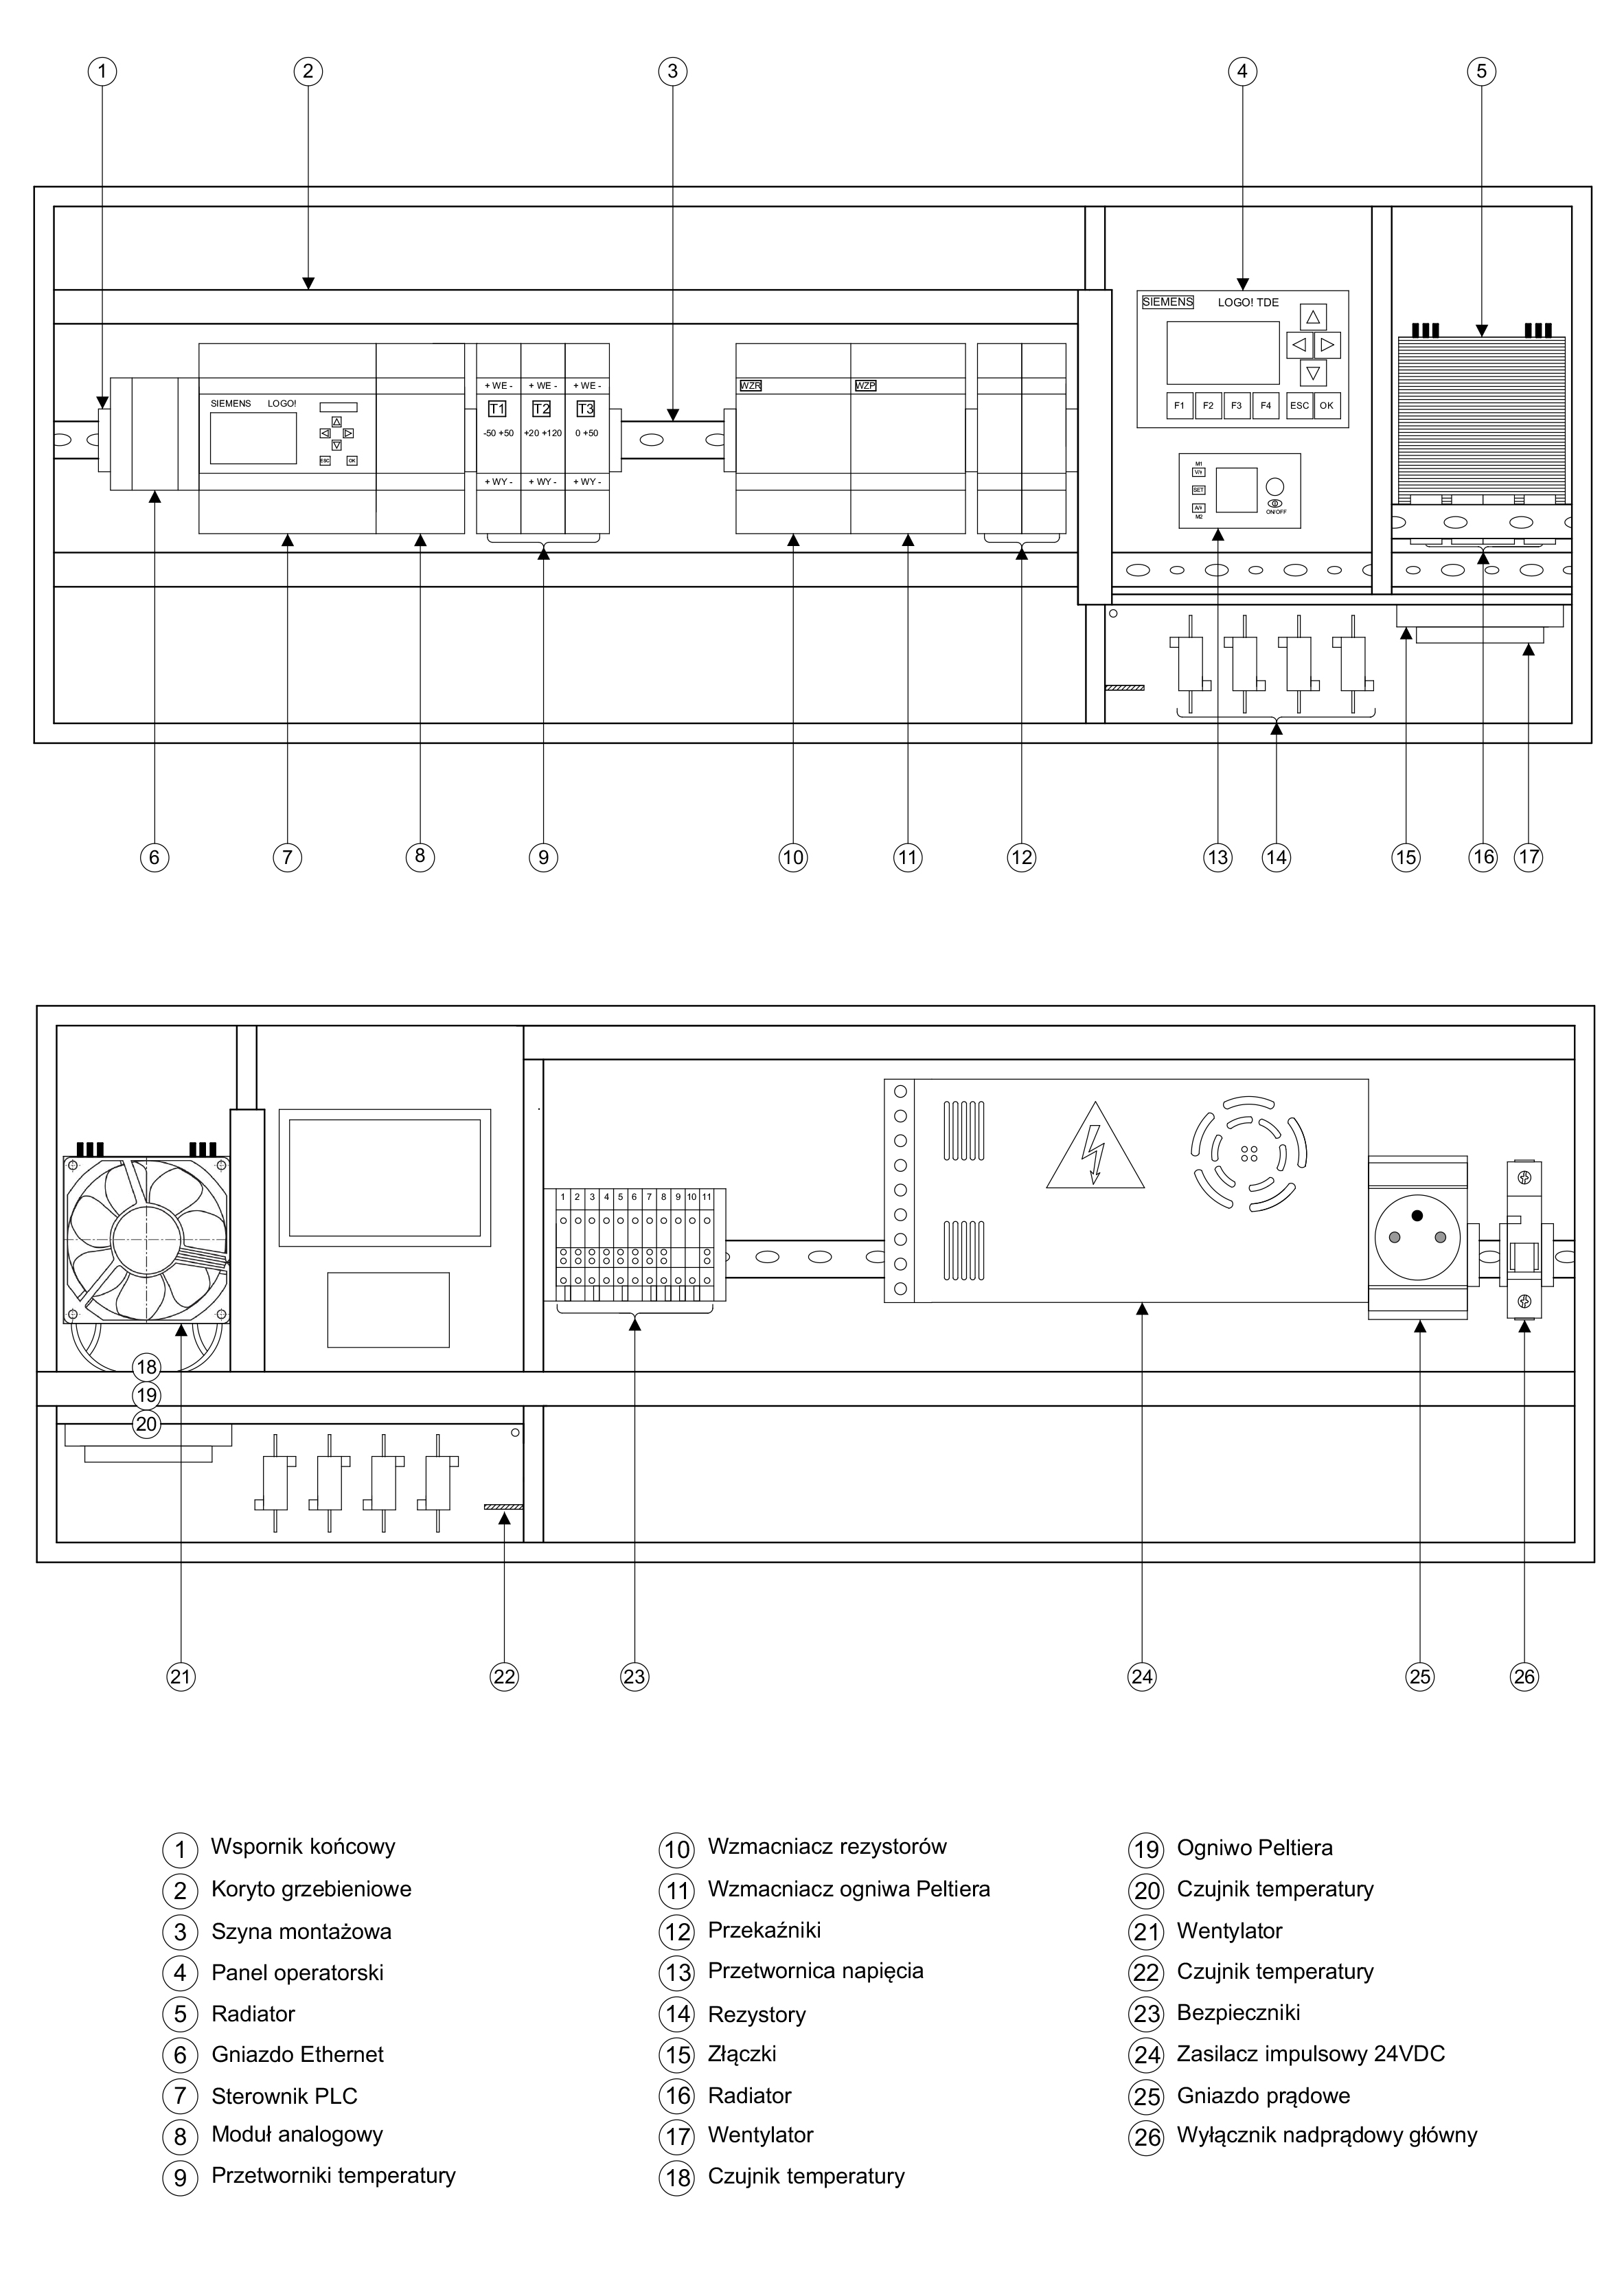
\includegraphics[width=\textwidth]{3.jpg}
    \caption{Schemat ideowy urządzenia}
\end{figure}

\section{Wykaz elementów}
Poniżej zostały przedstawione kolejno urządzenia odpowiedzialne za sterowanie układem, urządzenia wykonawcze oraz urządzenia pomiarowe. Przedstawione również zostały sygnały które każde z urządzeń odbiera i generuje wraz z krótkim ich opisem.
\subsection{Urządzenia sterujące}
Do urządzeń sterujących układem zaliczany jest sterownik PLC: LOGO!8 wraz z modułem analogowym oraz przetwornica napięcia typu: DPS5015 pozwalająca manualnie ustawić napięcie i natężenie prądu płynącego przez badane ogniwo termoelektryczne. Dodatkowo w układzie zastosowany został panel operatorski LOGO! TDE pozwalający na odczytywanie bieżących pomiarów temperatury. Panel umożliwia również sterowanie układem w trybie ręcznym.

\subsubsection{LOGO! 0BA8 (LOGO! 12/24RCE)}
LOGO! jest uniwersalnym modułem logicznym firmy Siemens który pozwala na zintegrowanie sterowania wraz z zasilaniem oraz interfejsem modułów rozszerzeń. Również istnieje możliwość podłączenia opcjonalnego modułu wyświetlania tekstu(TDE).

\begin{figure}
    \centering
    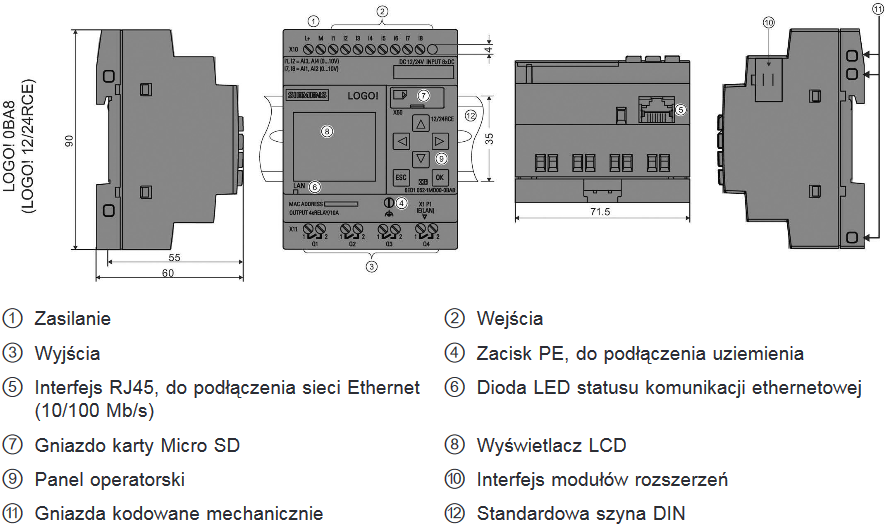
\includegraphics[width=\textwidth]{Sterownik_LOGO!.PNG}
    \caption{Sterownik LOGO! 0BA8 (LOGO! 12/24RCE)[3]}
\end{figure}

\subsubsection{LOGO! AM2 AQ (0/4\dots20 mA or 0 \dots 10 VDC)}
LOGO! AM2 AQ jest modułem analogowym zasilanym przez 24V DC. Posiada dwa wyjścia analogowe 4-20ma lub 0-10 VDC. W pracy moduł został wykorzystany do regulacji mocy rezystorów wewnątrz komory termicznej oraz regulacji prądu przepływającego przez ogniwo Peltira.

\begin{figure}
    \centering
    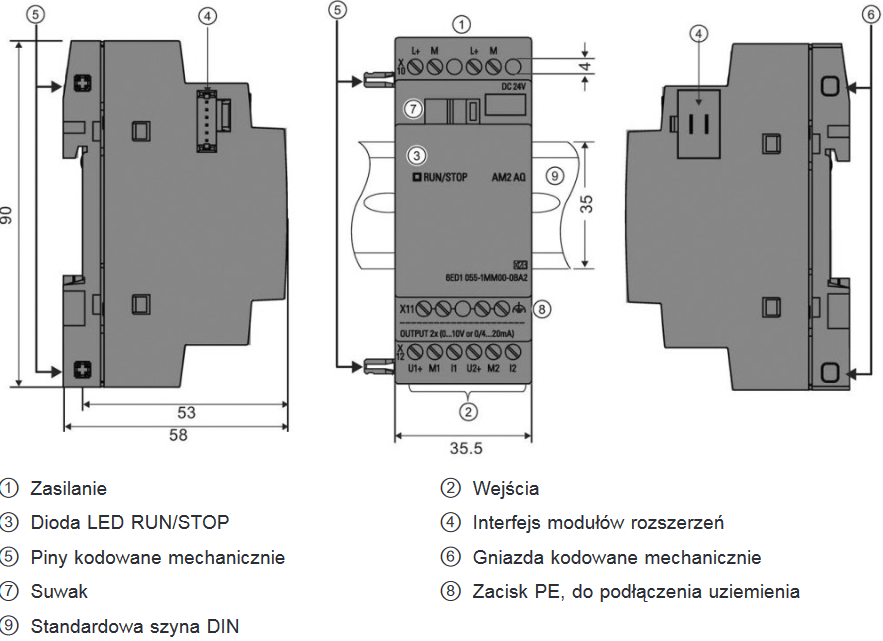
\includegraphics[width=\textwidth]{Modul_analogowy.PNG}
    \caption{Moduł analogowy LOGO! AM2 AQ (0/4\dots20 mA or 0 \dots 10 VDC)[3]}
\end{figure}

\subsubsection{Panel operatorski LOGO! TDE}

Użycie zintegrowanego z sterownikiem panelu operatorskiego LOGO! TDE pozwala na intuicyjne sterowanie całym układem. Sterowanie odbywa się przy pomocy czterech pulpitów operatorskich wykonanych w programie LOGO! SoftComfort. Panel operatorski posiada cztery przyciski funkcyjne, przyciski "ESC"i "ENTER" oraz cztery strzałki kierunkowe.

\begin{figure}
    \centering
    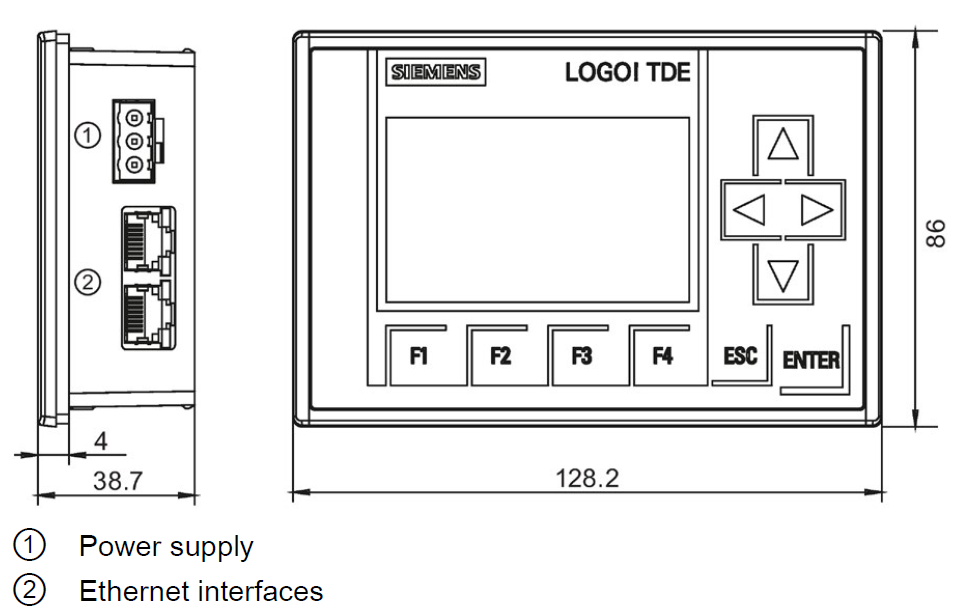
\includegraphics[width=\textwidth]{HMI.PNG}
    \caption{Panel operatorski LOGO! TDE [3]}
\end{figure}


\subsubsection{Przetwornica napięcia 0-50V 750W DPS5015}

Zasilacz DPS5015 oferuje bardzo wysoką precyzję i dokładność. Regulowane wyjście osiąga do 50V napięcia lub 15A natężenia i może być skonfigurowane w precyzyjnych krokach co 10mV lub 1mA. Zasilacz dodatkowo jest wyposażony w pamięć parametrów awaryjnego wyłączenia oraz programowalną pamięć danych. Urządzenie charakteryzuje się prostą obsługą, kolorowy wyświetlacz dostarcza podstawowych informacji między innymi mogą to być aktualne wartości napięcia i natężenia prądu wraz z mocą wyjściową[4].

\begin{figure}
    \centering
    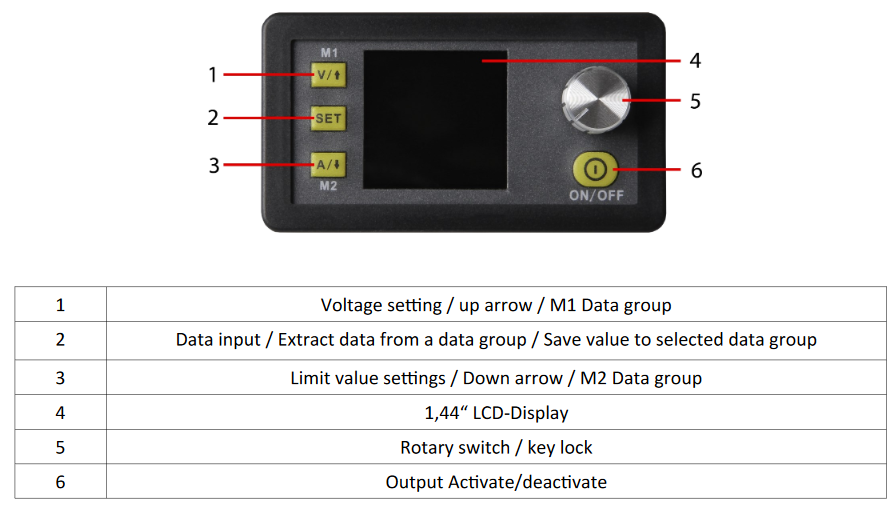
\includegraphics[width=\textwidth]{Przetwornica_napiecia.PNG}
    \caption{Przetwornica napięcia 0-50V 750W DPS5015[4]}
\end{figure}

\subsubsection{Analogowy wzmacniacz mocy}
Wzmacniacze wykorzystane w układzie służą do regulacji natężenia prądu płynącego przez moduł termoelektryczny oraz rezystory. Wykorzystany w obiekcie model wzmacniaczy to M12N3 pozwalają one na uzyskanie maksymalnego prądu pracy ciągłej 20A co w zupełności wystarcza do zasilenia zarówno rezystorów jak i ogniwa Peltiera. Pozwalają one na regulację mocy wyjściowej w zakresie 0-99\%. Wzmacniacz rezystorów jest zasilany bezpośrednio z zasilacza impulsowego prądu stałego. Wzmacniacz ogniwa Peltiera jest zasilany z przetwornicy napięcia. Wykorzystanie regulatorów zapewnia płynną regulację mocy wyjściowej charakteryzują się niezawodnością oraz małymi gabarytami.[15]

\subsection{Urządzenia wykonawcze}

Do grupy urządzeń wykonawczych wykorzystanych w projekcie które wpływają na temperaturę w komorze termicznej możemy zaliczyć: ogniwo Peltiera, przekaźniki, rezystory oraz radiatory wspomagane przez wentylatory. Dodatkowo w tej części zostały opisane elementy zasilające układ wraz z zastosowanymi urządzeniami bezpieczeństwa.
\subsubsection{Ogniwo Peltiera}
W układzie zastosowane zostało ogniwo Peltiera typu TEC1-12715. Nominalna wartość napięcia zasilania wybranego ogniwa wynosi 12 V(dopuszcza się napięcie do 15,5 V). Maksymalny pobór prądu wynosi natomiast 11.8 A co pozwala na pracę ogniwa z maksymalną odprowadzaną mocą do 142W. Ogniwo charakteryzuje się opornością od 0,8\ohm do 0,9\ohm.[13]
\subsubsection{Przekaźniki}
W pracy zostały użyte dwa przekaźniki RMP84 osadzone w gniazdach typu GZMB80. Pierwszy z nich został wykorzystany do przełączania kierunku przepływu prądu przez ogniwo Peltiera a tym samym zmianę polaryzacji na nim. Pozwala to na zmiany pracy ogniwa(grzanie, chłodzenie). Drugi przekaźnik pozwala na zmianę trybów pracy układu z ręcznego na automatyczny. Przekaźnik zapobiega również włączeniu dwóch trybów pracy jednocześnie i poboru prądu przez ogniwo jednocześnie z sterownika i zadajnika prądowego. Wybrano gniazda przekaźnikowe wyposażone w diody które zapobiegają "cofaniu" się prądu z układu na sterownik w momencie gdy np. układ zostanie wyłączony a temperatury strony zimnej i ciepłej ogniwa będą znacznie się różnić. W takim wypadku diody powodują rozproszenie się prądu.[12]
\subsubsection{Wentylatory}
W układzie zastosowane zostały dwa wentylatory firmy Saunon. Większy do wspomagania odprowadzania ciepła z radiatora strony ciepłej układu oraz mniejszy do strony zimnej układu. Oba wentylatory zasilane są przy pomocy dwóch przewodów napięciem 24V i generują 34 dBA hałasu. Większy wentylator pracuje z prędkością obrotową wynoszącą 2200 RPM co pozwala na przetłaczanie 127.3 $m^3/h$ powietrza. Mniejszy natomiast wspomagający odprowadzenie zimnego powietrza z ogniwa oraz rozprowadzenie go po komorze termicznej pracuje z prędkością obrotową wynoszącą 3000 RPM i wydajnością wynoszącą 87.4 $m^3/h$[8][9].
\subsubsection{Radiatory}
Do odprowadzenia ciepła ze strony grzejącej ogniwa oraz zimna ze strony chłodnej wykorzystano dwa żeberkowe radiatory wykonane z aluminium. Do odprowadzania ciepła ze strony gorącej ogniwa wykorzystano radiator SilentiumPC Fera 3. Radiator został wykonany z wykorzystaniem technologi HE (High Efficiency) wyposażony jest w cztery rurki cieplne które dotykają bezpośrednio modułu i tym samym poprawiają odprowadzanie ciepła zapewniając niższe temperatury. Wykorzystany radiator pozwala na odprowadzenie 180W mocy cieplnej co w zupełności wystarcza dla zastosowanego ogniwa Peltiera. Do rozprowadzania chłodu wewnątrz komory termicznej użyto prostego radiatora żeberkowanego[14]. 
\subsubsection{Rezystory}
W celu wprowadzenia zakłóceń do układu w komorze termicznej zostały zamontowane cztery przykręcane rezystory drutowe zintegrowane z radiatorami. Każdy charakteryzuje się mocą 50W i opornością 20\ohm. Wszystkie rezystory zostały połączone równolegle i w pracy traktowane są jako jedno źródło ciepła. Regulacji temperatury na rezystorach dokonuje się manualnie przy użyciu panelu operatorskiego TDE lub automatycznie przy pomocy sterownika PLC[10].
\subsubsection{Zasilanie}
Zasilanie układu zostało zrealizowane przy pomocy stabilizowanego impulsowego zasilacza 24V - 20A - 480W. Wykorzystany zasilacz charakteryzuje się małymi gabarytami w porównaniu do innych transformatorowych zasilaczy oraz  dużą stabilnością napięcia wyjściowego. Dodatkowo na szynie obok zasilacza zostało zamontowane gniazdo elektryczne.
\subsubsection{Bezpieczeństwo}
W układzie został zamontowany główny wyłącznik nadprądowy TDZ 16A charakterystyka B. Koniecznością było zastosowanie wyłącznika 8A z uwagi na natężenie prądu pobierane przez ogniwo i moce jakie generuje. Dodatkowo każdy z rezystorów oraz urządzenia sterujące zostały zabezpieczone przez  bezpieczniki szklane typu F2AL250V. Ogniwo Peltiera dodatkowo zabezpiecza szklany bezpiecznik zwłoczny typu T10AL250V. Wszystkie bezpieczniki szklane zostały zainstalowane w dedykowanych kasetach.[11]

\subsection{Urządzenia pomiarowe}
Urządzeniami mierzącymi w czasie rzeczywistym temperaturę zimnej i ciepłej strony modułu wraz z temperaturą wewnątrz komory termicznej są czujniki temperatur typu: PT0-10. 

PT0-10 składa się z układu cyfrowego przetwornika sygnału na napięcie 0-10V oraz czujnika temperatury DS18B20. Sygnał wyjściowy przetwornika jest proporcjonalny do mierzonej przez czujnik temperatury. Zespół urządzeń PT0-10 pozwala na ograniczenie zakresu mierzonej temperatury do interesujących nas granic pomiarowych. Taki zabieg pozwala zwiększyć rozdzielczość dokonywanych pomiarów w określonym przedziale temperaturowym. Czujnik temperatury T0-92 jest połączony z przetwornikiem przy pomocy trójżyłowego kabla o długości dwóch metrów który można dodatkowo przedłużyć lub skrócić do maksymalnie 0,2m na potrzeby projektu. Jeśli połączenie czujnika z przetwornikiem będzie dłuższe niż 5m powinno być ono dodatkowo ekranowane oraz uziemione w celu minimalizacji zakłóceń pomiarowych na sygnał analogowy. Do wykonywania długich połączeń czujnika z z przetwornikiem producent zaleca stosowanie skrętki z koralikiem ferrytowym. Płytka przetwornika została zamontowana w dedykowanej obudowie typu KMz-105[6].

W zbudowanym urządzeniu zostały wykorzystane trzy układy pomiaru temperatury PT0-10:
\begin{itemize}
    \item T1 - Czujnik umieszczony bezpośrednio pod ogniwem Peltiera pozwalający na pomiar temperatury zimnej strony ogniwa. Zakres mierzonych temperatur wynosi -50\dots50 stopni C przy dokładności pomiaru wynoszącej 0,1 stopnia.
    \item T2 - Czujnik umieszczony bezpośrednio nad ogniwem Peltiera pozwalający na pomiar temperatury gorącej strony ogniwa. Zakres mierzonych temperatur wynosi 20\dots120 stopni C przy dokładności pomiaru wynoszącej 0,1 stopnia.
    \item T3 - Czujnik umieszczony wewnątrz komory termicznej. Zakres mierzonych temperatur wynosi 0\dots50 stopni C przy dokładności pomiaru wynoszącej 0,05 stopnia.
\end{itemize}
Wszystkie układu pomiarowe zasilane są napięciem 24V z sterownika PLC.
\newpage
\begin{table}[h!]
\footnotesize
\begin{tabularx}{\textwidth}{|c|X|X|c|c|}
\hline
\rowcolor{lightgray}
    Lp. & \multicolumn{2}{|c|}{Urządzenie}        & Ilość          & Producent                                    \\\hline
    1.      &LOGO!8 12/24RCE     &Sterownik PLC      &1       &Siemens\\\hline
    2.      &LOGO!8 AM2 AQ-6ED1055-1MM00-0BA2    &Moduł analogowy      &1       &Siemens\\\hline
    3.      &LOGO! TDE    &Panel operatorski      &1       &Siemens\\\hline
    4.      &M12N3    &Wzmacniacz      &2       &CAY Regulatory\\\hline
    5.      &PT0-10    &Czujnik temperatury z przetwornikiem      &3       &Telematic\\\hline
    6.      &DPS5015    &Przetwornica napięcia      &1       &Gotronik\\\hline
    7.      &TEC1-12715    &Ogniwo Peltiera      &1       &Hesta\\\hline
    8.      &24V-20A-480W     &Zasilacz impulsowy     &1       & 	nieokreślony\\\hline
    9.      &RMP84 2012-25-1024-WT      &Przekaźnik     &2       &Relpol\\\hline
    10.      &GZMB80      &Gniazdo przekaźnika     &2       &Relpol\\\hline
    11.      &1F TYP S301 B-16A     &Wyłącznik główny nadprądowy     &1       &Tracon Electric\\\hline
    12.      &F2AL250V      &Bezpiecznik szklany szybki     &5       &Elektropark\\\hline
    13.      &T10AL250V      &Bezpiecznik szklany zwłoczny     &1      &Elektropark\\\hline
    14.      &TS-35 z otwor. 35x7,5x1000mm      &Szyna montażowa     &2      &EBMiA\\\hline
    15.      &PR-0478     &Koryto grzebieniowe 25x25/2000mm     &1      &EBMiA\\\hline
    16.      &PR-0668    &Koryto grzebieniowe 25x40/2000mm     &1      &EBMiA\\\hline
    17.      &3842992888/3000    &Profil, materiał: aluminium, dł. 3000mm, 20 x 20 mm   &1      &Bosch Rexroth\\\hline
    18.      &3842535572   &Klamra, 10mm     &32      &Bosch Rexroth\\\hline
    19.      &3842530285    &Nakrętka do rowków typu T, 10mm     &10      &Bosch Rexroth\\\hline
    20.      &EW 35-383560000    &Wspornik końcowy   &8      &Weidmuller\\\hline
    21.      &1061200000    &Wspornik końcowy   &4      &Weidmuller\\\hline
    22.      &1763940000 WTR 2.5/SI    &Zaciskowa złączka szynowa   &4      &Weidmuller\\\hline
    23.      & WSI 6/LD 10-36V DC/AC -1011300000     &Złączka szynowa bezpiecznikowa   &7      &Weidmuller\\\hline
    24.      &2ESDV-06P; 6 torów     &Łączówka   &2      &Dinkle\\\hline
    25.      &2EHDRD-08P     &Złączka   &2      &Dinkle\\\hline
    26.      &2m$^2$ grubość 6mm    &Plexi bezbarwna   &1      &Folplex\\\hline
    27.      &Z106    &Obudowa \newline wzmacniacza   &2      &KRADEX\\\hline
    28.      &KMz 105    &Obudowa przetwornika temperatury   &3      &MASZCZYK\\\hline
    29.      &4520041    &Kabel 1,5mm$^2$ czerwony - 10m  &1      &Lapp\\\hline
    30.      &4510013    &Kabel 1mm$^2$ czarny - 10m  &1      &Lapp\\\hline
    31.      &4510012   &Kabel 0,75 mm$^2$ czarny - 10m  &1      &Lapp\\\hline
    \pagebreak
    32.      &4510042  &Kabel 0,75 mm$^2$ czerwony - 10m  &1      &Lapp\\\hline
    33.      &RH05020R00FE02  &Rezystor drutowy 50W20\ohm  &4      &Vishay\\\hline
    34.      &SPC144  &Radiator strony grzejącej  &1      &SilentiumPC\\\hline
    35.      &A5724/10  &Radiator strony zimnej &1      &Kęty\\\hline
    36.      &EE92252B1-A99  &Wentylator wewnętrzny  &1      &Sunon\\\hline
    37.      &EEC0252B3-A99  &Wentylator zewnetrzny  &1      &Sunon\\\hline
    38.      &FBA\_180031x5  &Gniazdo Ethernet &1      &Cable Matters \\\hline
    39.      &DMM3ZW6 M3 L=6mm  &Dystans  &8      &nieokreślony\\\hline
    40.      &D-Sub; Canon 9p  &Odgiętka  &2      &nieokreślony\\\hline
    41.      &002414010  &Gniazdo modułowe 2P+Z 10/16A 230V &1      &EVE\\\hline
    
    
\end{tabularx}
   \caption{Spis elementów}
\end{table}

\section{Uruchomienie i obsługa urządzenia}
\subsection{Uruchomienie urządzenia}
Poniżej został przedstawiony schemat postępowania w celu uruchomienia urządzenia:
\begin{enumerate}
    \item Podłączenie obiektu do źródła prądu przemiennego 230V przy pomocy przewodu zasilającego.
    \item Włączyć cały układ przy pomocy zmiany pozycji dźwigni głównego bezpiecznika  znajdującego się z tyłu urządzenia. Po wykonaniu tej czynności powinniśmy zauważyć uruchomienie się sterownika PLC w tryb "run" oraz uruchomienie panelu HMI oraz ekranu zadajnika prądowego.
    \item Zewnętrzy komputer podłączyć do urządzenia przy pomocy przewodu ethernet.
    \item Uruchomić specjalistyczne oprogramowanie i połączyć się z urządzeniem.
    \item Urządzenie jest gotowe do działania.
\end{enumerate}

\subsection{Obsługa programowalnego modułu zasilania}
\subsubsection{Ekran główny}
Po włączeniu zasilania na wyświetlaczu urządzenia można zauważyć ekran powitalny następnie moduł zasilający przechodzi do głównego okna, które zawiera podstawowe informacje takie jak: natężenie wyjściowe, napięcie wyjściowe oraz moc. Nad podstawowymi informacjami znajduje się ustawione napięcie oraz natężenie prądu. Istnieje możliwość zmiany tych wartości poprzez wciśnięcie przycisku $M1$ w przypadku zmiany napięcia i $M2$ w przypadku zmiany natężenia prądu. Można zwiększać wartości poruszając potencjometrem zgodnie z wskazówkami zegara i zmniejszać obracając go w drugą stronę. Ponowne wciskanie potencjometru pozwala na zmianę dokładności ustawianych wartości kolejno do wartości dziesiętnych i setnych. Akceptacji ustawionych wartości dokonuje się przez ponowne naciśnięcie przycisku $M1$ w przypadku zmiany napięcia i $M2$ w przypadku zmiany natężenia prądu. Informacja o napięciu jakie jest podawane na wejście urządzenia znajduje się u dołu ekranu. Po prawej stronie ekranu znajdują się ikony stanu pracy, ikona blokady klawiszy, ikona stanu nieprawidłowego wyjścia, wskaźnik stanu pracy CV(stabilizacja napięcia) lub CC(stabilizacja prądu) oraz ikona wyjścia włączone/wyłączone. Włączenie i wyłączenie urządzenia następuje po wciśnięciu przycisku $ON/OFF$.

\textbf{UWAGA!} Należy pamiętać o włączeniu funkcji sterowania ręcznego w celu ustawiania napięcia oraz natężenia prądu dla ogniwa Peltiera przy pomocy zadajnika prądowego.
\subsubsection{Zmiana napięcia i natężenia prądu wyjściowego}
Aby dokonać zmiany napięcia lub natężenia prądu należy przycisnąć przycisk $SET$. Po wciśnięciu przycisku następuje przejście do ekranu zmiany danych. Następnie przy pomocy przycisków $M1$ oraz $M2$ wybieramy parametr do zmiany:
\begin{itemize}
    \item U-SET - napięcie prądu wyjściowego,
    \item I-SET - natężenie prądu wyjściowego,
    \item S-OVP - górna granica napięcia na wyjściu,
    \item S-OCP - górna granica wartości natężenia na wyjściu,
    \item S-OPP - górna granica wartości mocy na wyjściu,
    \item B-LED - ustawienie jasności wyświetlacza,
    \item M-PRE - ustawienie komórki pamięci(10 możliwości).
\end{itemize}
Po wybraniu parametru do zmiany należy nacisnąć pokrętło potencjometru. Po wciśnięciu pokrętła zostaje podświetlona wartość która podlega zmianie. Obracając pokrętło potencjometru zgodnie z wskazówkami zegara powodujemy zwiększenie wartości zmienianej, w przeciwną stronę powodujemy jej obniżenie. Kolejne przyciśnięcia pokrętła pozwalają na zmianę dokładności ustawianej wartości kolejno o liczby dziesiętne i setne. Aby zaakceptować wybraną wartość należy wcisnąć przycisk $SET$ bądź poczekać 1min. Po tym czasie wartość zostanie automatcznie zapisana.
\subsubsection{Zapisywanie grupy ustawionych danych}
Istnieje możliwość zapisania w pamięci urządzenia grupy ustawionych danych. Aby tego dokonać należy po wciśnięciu przycisku $SET$ w ekranie głównym przejść do pozycji $M-PRE$. Następnie należy wcisnąć pokrętło potencjometru i obracając nim wybrać wolny slot pamięci $M0\dots M9$. Po wybraniu wolnego slotu należy ponownie wcisnąć potencjometr i ustawić wartość $ON$.

\chapter{Oprogramowanie}
\section{LOGO! SoftComfort}
Pakiet LOGO! SoftComfort pozwala na wygodne programowanie w jednym środowisku programistycznym sterowników serii: LOGO! oraz współpracujących z nimi paneli operatorskich i innych urządzeń producenta. Pakiet oprogramowania zawiera wiele udogodnień i rozwiązań ułatwiających pracę z sterownikami. Między innymi posiada przejrzysty interfejs graficzny pozwalający na pracę bez konieczności posługiwania się samym urządzeniem LOGO!. Program napisano przy pomocy bloków funkcjonalnych (Function Block) jednakże LOGO! SoftComfort pozwala również na programowanie języku drabinkowym.

Dodatkowym udogodnieniem jest możliwość symulacji działania całego układu w komputerze PC. Program również można testować online co daje możliwość podejrzenia zmian stanów wejść i wyjść cyfrowych oraz zmiennych procesowych w trybie sterownika "RUN". Przenoszenie napisanego programu z komputera PC do sterownika PLC i odwrotnie odbywa się przy pomocy przewodu Ethernet.

\section{Baza danych pomiarowych}
Wykorzystanie pakietu Microsoft Office a konkretnie programu Excel pozwala na utworzenie prostej bazy danych. Program Excel do poprawnej pracy z sterownikiem PLC wymaga pobrania narzędzia LOGO!AccessTool dostępnego na stronie Siemensa. Następnie należy zaimportować dodatek LOGO!AccessTool do programu Excel i go skonfigurować miedzy innymi określić w jakich odstępach czasowych dane mają być pobierane z sterownika.  Poprawna instalacja i konfiguracja narzędzia pozwala na odczyt i zapis danych z czujników pomiarowych w czasie rzeczywistym. 

Dzięki pakietowi office jest możliwa również dalsza interpretacja zebranych pomiarów. Program Excel daje możliwość utworzenia tabel czy wykresów. Analiza i badanie zebranych danych pomiarowych z obiektu jest przedstawiona w dalszej części pracy.

\chapter{Badanie ogniwa Peltiera}

Głównym elementem układu badawczego jest półprzewodnikowy moduł Peltiera, który jest zasilany z zadajnika prądowego wykorzystanego w układzie. Bezpośrednio nad i pod modułem Peltiera zostały umieszczone bloki aluminiowe będące ośrodkami magazynującymi ciepło. Wewnątrz aluminiowych bloków osadzono dwa czujniki temperatury. Czujnik umieszczony w górnym bloku aluminiowym służy do pomiaru ciepła wydzielanego przez stronę gorącą ogniwa natomiast czujnik umieszczony w dolnym bloku mierzy ciepło pobierane z komory chłodniczej.Moduł został osadzony na radiatorze chłodzonym przy pomocy wentylatora. Wykorzystanie radiatora wspomaganego przez wentylator po stronie zimnej zwiększa całkowite "pompowanie" ciepła przez moduł Peltiera. Ze względu na charakterystykę ogniwa Peltiera na zadajniku prądowym ustalono ograniczenie napięcia wynoszące 15V co zapobiega spaleniu się termoelementu.

Dane zmierzone przez czujniki temperatury były zapisywane w odstępach czasowych wynoszących 1s i zapisywane do bazy danych opisanej w rozdziale trzecim. Badania rozpoczęto od ustawienia natężenia prądu na 1A a następnie przez kolejno 60s, 120s, 180s zbierano dane z czujników temperatury. Po minięciu czasu wykonywania pomiarów próbka absorbująca ciepło w postaci bloku aluminiowego była chłodzona do temperatury początkowej z dokładnością wynoszącą 0,5 stopnia. Badania powtórzono zwiększając natężenie prądu po każdym badaniu o 1A dla wartości natężenia prądu od 1A do 10A zwiększając natężenie prądu po każdym badaniu o 1A.


Badania przeprowadzone na module Peltiera opisane w tym rozdziale zostały przeprowadzone w oparciu o artykuły naukowe[16][17].
\newpage
\section{Model matematyczny}
Przewodzenie cieplne zależne od czasu można zauważyć w momencie gdy pewne ciało doświadcza nagłej zmiany środowiska termicznego. Jeśli badane ciało jest małe wtedy gradienty temperatury w ciele można pominąć. W tabeli przedstawione zostały stałe charakteryzujące zastosowany w celu badań blok aluminiowy:
\\
\begin{center}
\begin{figure}[h!]
    \centering
    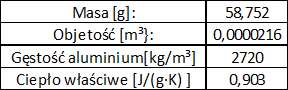
\includegraphics[width=5cm]{Blok_aluminiowy_dane.png}
    \captionof{table}[Charakterystyka bloku aluminiowego]{Charakterystyka bloku aluminiowego}
    \end{figure}
\end{center}

Badanie takiego ciała i jego zmiany temperatury zależnie od czasu można badać przy wykonaniu ogólnego bilansu ciepła elektrycznego:
\begin{equation}
    \dot{E_{we}} = \dot{E_{zm}}
\end{equation}
gdzie:\\
$\dot{E_{we}}$ -moc generowana przez moduł Peltiera, \\
$\dot{E_{zm}}$ - moc zmagazynowana przez blok aluminiowy. \\

Na podstawie definicji transportu cieplnego:
\begin{equation}
    \dot{E_{we}} = mc \frac{dT}{dt} = \rho Vc \frac{dT}{dt}
\end{equation}
gdzie:\\
$m$ - masa bloku, \\
$c$ - ciepło właściwe, \\
$dT$ - zmiana temperatury, \\
$dt$ - zmiana czas \\
$\rho$ - gęstość, \\
$V$ - objętość. \\

\section{Badanie efektu Joul'a}
Efekt Joul'a nazywany jest również zjawiskiem Joul'a-Lenza. Zjawisko to opisuje zamianę energii elektrycznej na energię cieplną podczas przepływu prądu przez opornik. Ciepło Joul'a $Q_J$ wytwarza się podczas przepływu prądu przez ogniwo Peltiera będące opornikiem o rezystancji 0,88\ohm.
\begin{equation}
    Q_J = I^2 \cdot R
\end{equation}
gdzie:\\
$Q_J$ - ciepło Joul'a,\\
$I$ - Natężenie prądu elektrycznego,\\
$R$ - oporność ogniwa Peltirera.

\newpage
W poniższej tabeli zostało przedstawione obliczone ciepło Joul'a $Q_J$ w zależności od podanego na moduł Peltiera natężenia prądu elektrycznego. Wyniki przedstawione w tabeli zostały zilustrowane na rysunku.
\begin{center}
\begin{figure}[h!]
    \centering
    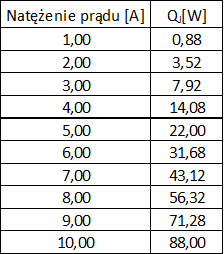
\includegraphics[width=5cm]{QJ_dane.png}
    \captionof{table}[Obliczona moc Joul'a]{Obliczona moc Joul'a}
    \end{figure}
\end{center}
\begin{center}
\begin{figure}[h!]
    \centering
    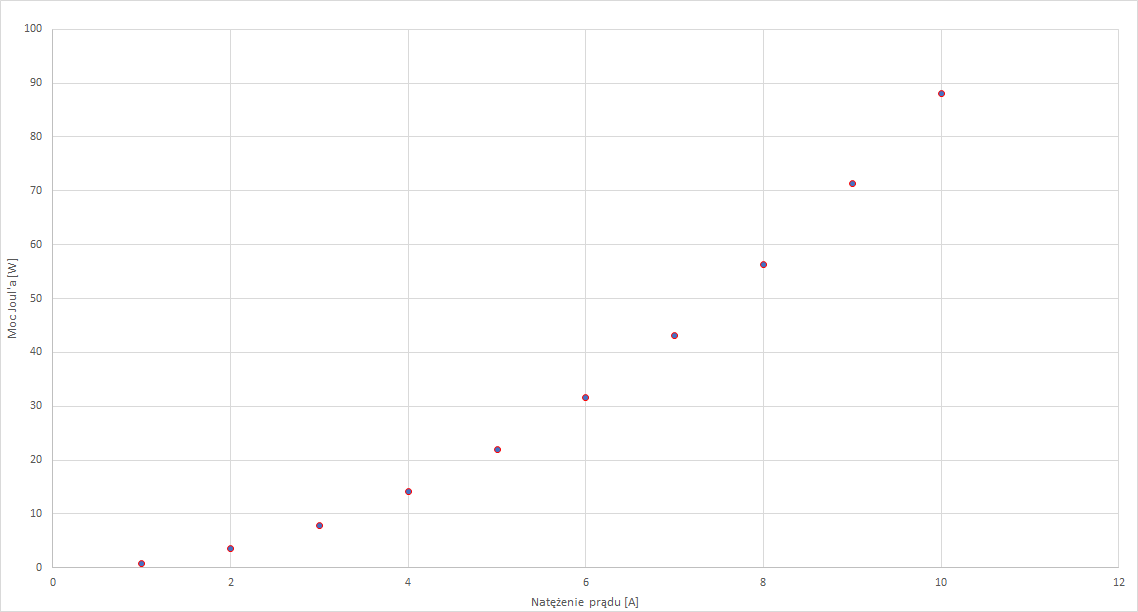
\includegraphics[width=\textwidth]{QJ_wykres.png}
    \caption{Zależność mocy Joul'a od natężenia prądu}
    \end{figure}
\end{center}
\newpage
\section{Wyznaczenie mocy modułu Peltiera}
Zgodnie z równaniem bilansu cieplnego(5.2) niezbędne do wyznaczenia mocy grzewczej modułu Peltiera jest obliczenie zmiany temperatury w bloku aluminiowym w zależności od czasu($\frac{dT}{dt}$). Wyniki przedstawiające zmianę temperatury w czasie zostały mierzone w odstępach czasowych wynoszących 1s i zapisywane w bazie danych. Zmierzone wartości zostały zilustrowane na rysunku 5.2. Na podstawie uzyskanego wykresu można wywnioskować, że dla wszystkich badanych natężeń prądu w miarę upływu czasu wytwarzanie ciepła przez moduł Peltiera stabilizuje się na określonym poziomie. Niedokładności pomiarowe przy wyższych natężeniach prądu spowodowane są brakiem pełnej izolacji badanego modułu Peltiera oraz narastającą wraz z zwiększaniem prądu mocy Joul'a($Q_J$).

\begin{center}
\begin{figure}[h!]
    \centering
    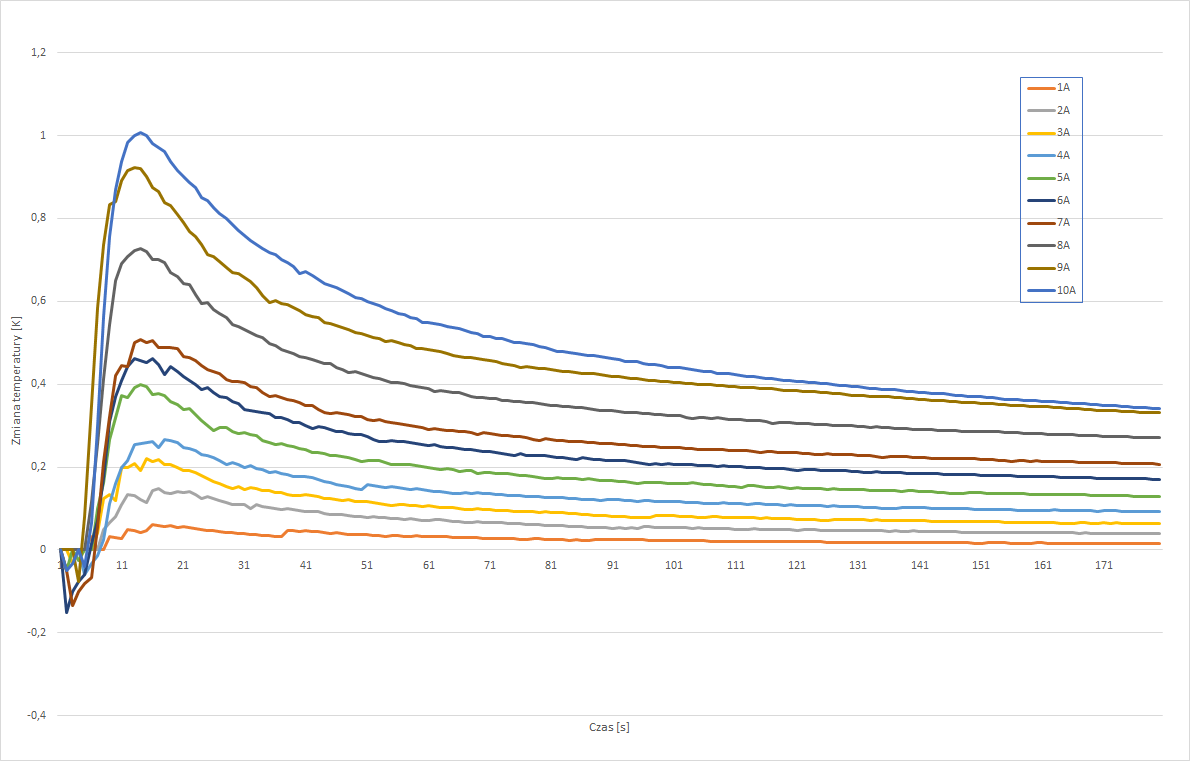
\includegraphics[width=\textwidth]{Qg_wykres.png}
    \caption{Wykres zmiany temperatury w czasie w aluminiowym bloku[dT/dt]}
    \end{figure}
\end{center}

Wykorzystując zmierzone dane przedstawione na rysunku 5.2 oraz dane charakteryzujące blok aluminiowy przedstawione w tabeli 5.1 obliczono na podtawie wzoru $Q_g = mc \cdot \frac{dT}{dt}$  moc transferowaną do bloku aluminiowego(moc grzania). Obliczone moce w zależności od natężenia prądu zostały przedstawione w tabeli 5.3 i zilustrowane na rysunku 5.3.

\begin{center}
\begin{figure}[h!]
    \centering
    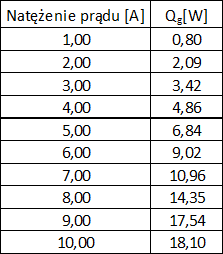
\includegraphics[width=5cm]{Qg_dane.png}
    \captionof{table}[Ciepło wygenerowane w bloku aluminiowym w czasie 180s]{Ciepło wygenerowane w bloku aluminiowym w czasie 180s}
    \end{figure}
\end{center}

\begin{center}
\begin{figure}[h!]
    \centering
    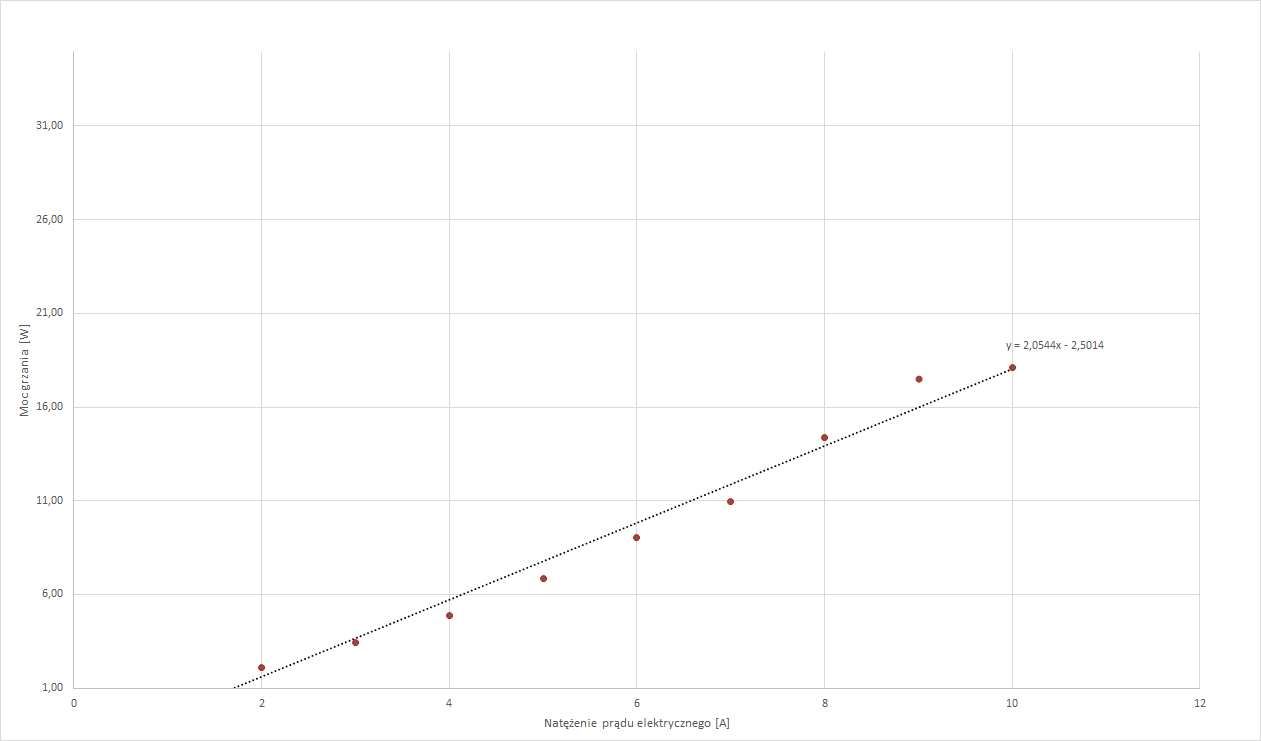
\includegraphics[width=\textwidth]{Qgrzanie_wykres.png}
    \caption{Moc grzania w zależności od natężenia prądu}
    \end{figure}
\end{center}

\section{Wyznaczenie sprawności modułu Peltiera}
Ważnym parametrem badanego modułu jest jego sprawność. Aby obliczyć sprawność wykorzystanego modułu jako pompy ciepła należy skorzystać ze wzoru:
\begin{equation}
    \eta = \frac{Q_g}{P_{el}}
\end{equation}
W chwili czasu w której nastąpiło ustabilizowanie przyrostu temperatury w czasie w badanym bloku aluminiowym ($\frac{dT}{dt} = const$) odczytano napięcie i natężenie prądu podawane na moduł termoelektryczny. Na podstawie odczytanych danych obliczono moc podawaną na moduł przez zadajnik prądowy korzystając ze wzoru na moc elektryczną.
\begin{equation}
    P_{el} = U \cdot I
\end{equation}
gdzie: \\
$P_{el}$ - moc elektryczna podawana na ogniwo przez zadajnik prądowy, \\
$U$ - napięcie prądu odczytane z zadajnika, \\
$I$ - ustawione natężenie prądu. \\

Wyniki przedstawiające zależność obliczonej mocy elektrycznej podawanej na ogniwo od natężenia prądu zostały przedstawione w tabeli 5.4 i zaprezentowane na rysunku 5.4.
\begin{center}
\begin{figure}[h!]
    \centering
    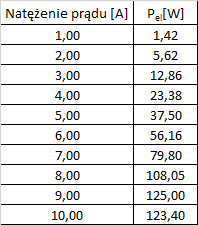
\includegraphics[width=5cm]{Pel_dane.png}
    \captionof{table}[Moc elektryczna podawana na ogniwo w czasie t = 180s]{Moc elektryczna podawana na ogniwo w czasie t = 180s}
    \end{figure}
\end{center}

Moc podawana na moduł Peltiera w zależności od natężenia prądu daję się przybliżyć wielomianem drugiego stopnia. Równanie zostało przedstawione na rysunku.

\begin{center}
\begin{figure}[h!]
    \centering
    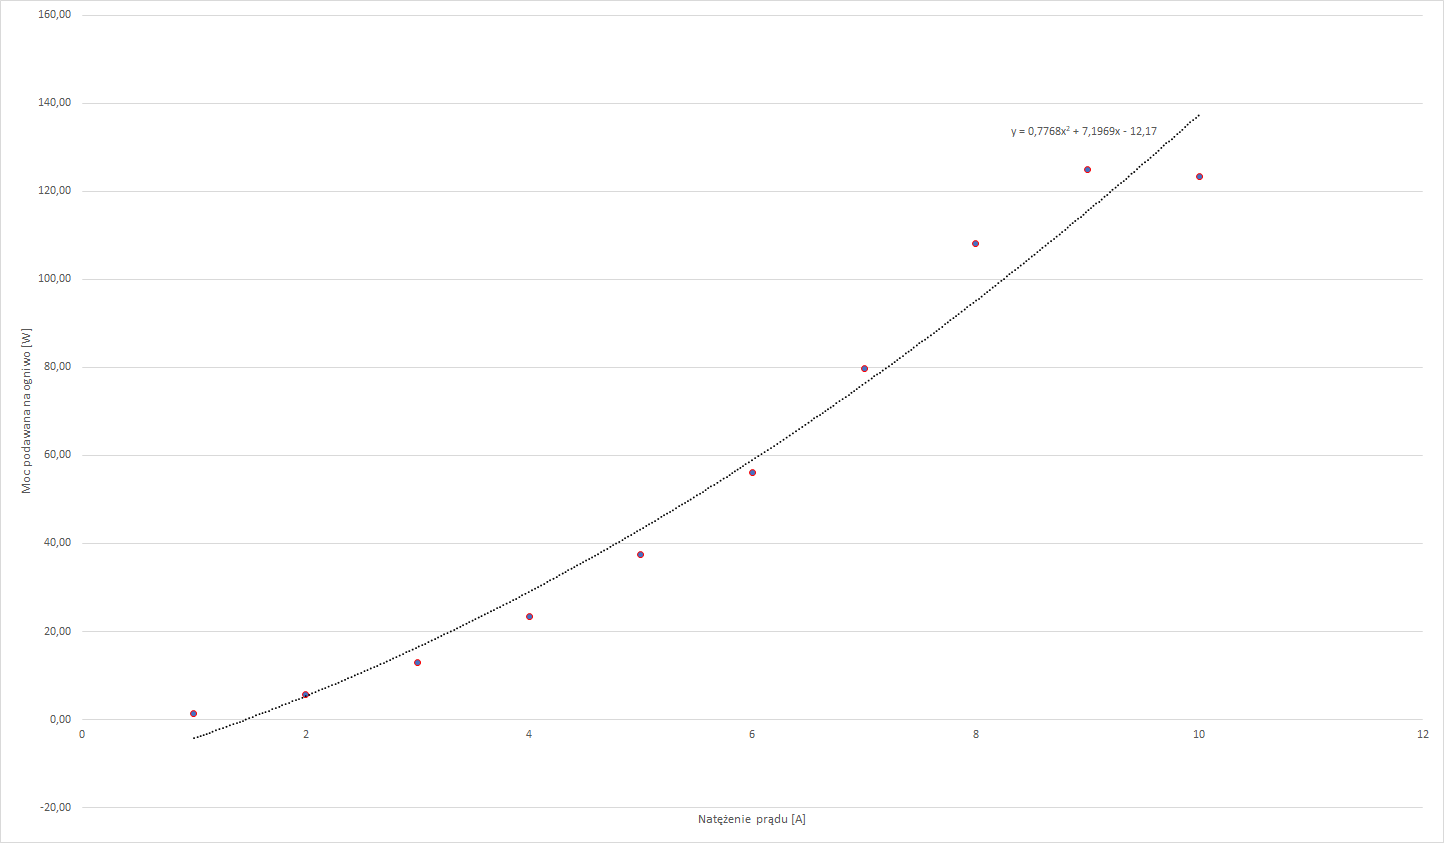
\includegraphics[width=\textwidth]{Pel_wykres.png}
    \caption{Zależność mocy podawanej na moduł Peltiera od natężenia prądu}
    \end{figure}
\end{center}

Na podstawie obliczonej mocy elektrycznej podawanej na moduł Peltiera oraz wzoru (5.4) wyznaczono sprawność modułu od podawanego na niego prądu elektrycznego. Wyniki zostały przedstawione w tabeli 5.5.

\begin{center}
\begin{figure}[h!]
    \centering
    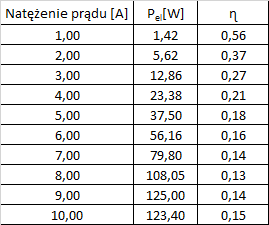
\includegraphics[width=5cm]{Spr_dane.png}
    \captionof{table}[Sprawność elektryczna modułu Peltiera w chwili t = 180s]{Sprawność elektryczna modułu Peltiera w chwili t = 180s}
    \end{figure}
\end{center}

\begin{center}
\begin{figure}[h!]
    \centering
    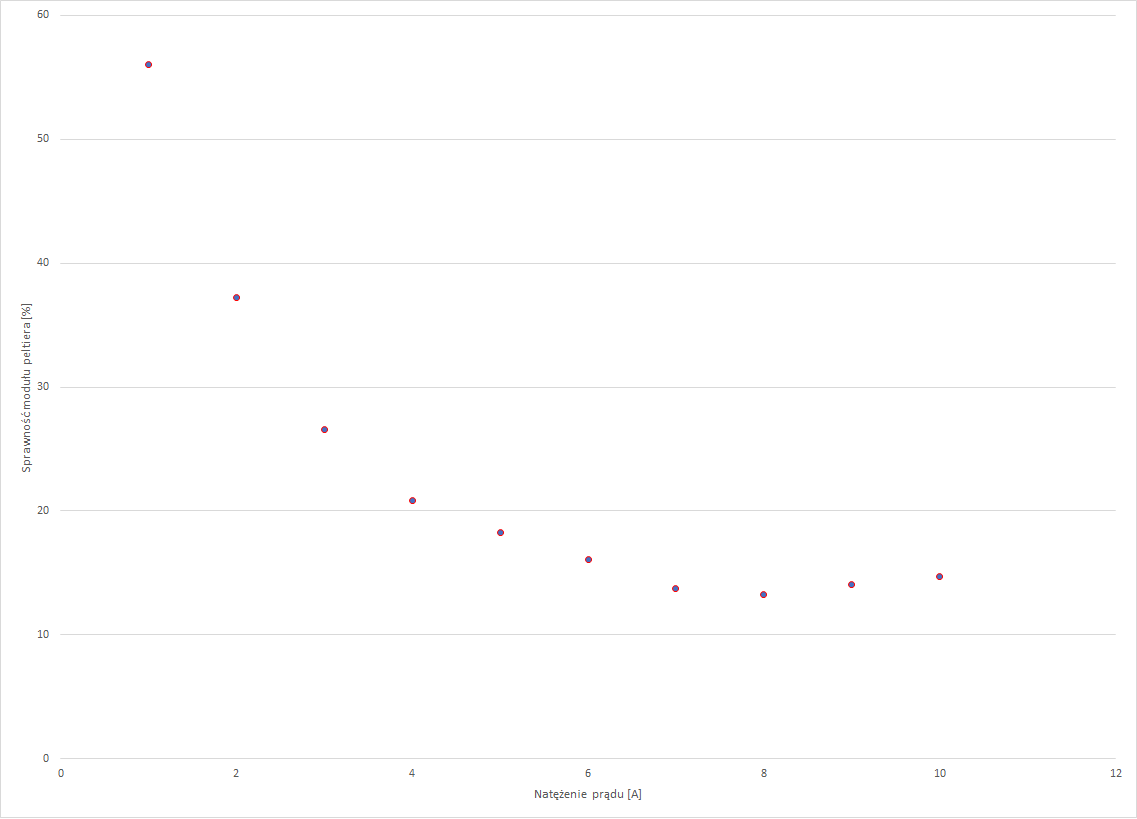
\includegraphics[width=\textwidth]{Spr_wykres.png}
    \caption{Sprawności modułu Peltiera jako pompy ciepła od natężenia prądu}
    \end{figure}
\end{center}
Na podstawie obliczonych danych oraz wykresu można wywnioskować ,że moduł Peltiera jako pompa ciepła charakteryzuje się wysoką sprawnością w niskich zakresach natężenia prądu. Na przykład dla 1A natężenia prądu sprawność modułu termoelektrycznego wynosi w przybliżeniu 56\%. W trakcie zwiększania prądu sprawność modułu maleje do około 14\%.


\section{Badanie efektywności chłodzenia modułem Peltiera w zależności od natężenia prądu}
Badanie efektywności chłodzenia modułem Peltiera przeprowadzono na podstawie zależności mocy chłodzącej od natężenia prądu podawanego na moduł. Moc chłodzącą można przedstawić jako całkowitą moc podawaną na moduł termoelektryczny pomniejszoną o wartości mocy grzania oraz mocy Joul'a.
\begin{equation}
    Q_c = P_{el}-Q_g-Q_J
\end{equation}
gdzie:\\
$Q_c$ - moc chłodzenia modułu Peltiera,\\
$P_{el}$ - moc elektryczna podawana na moduł,\\
$Q_g$ - moc grzania modułu, \\
$Q_J$ - moc Joul'a. \\

Wartości mocy chłodzenia od natężenia prądu przedstawia poniższa tabela i rysunek.
\begin{center}
\begin{figure}[h!]
    \centering
    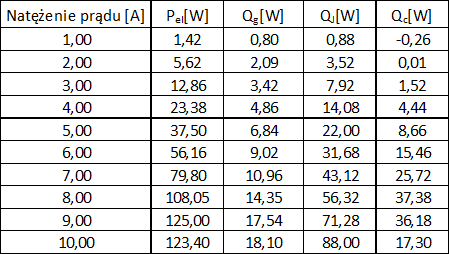
\includegraphics[width=10cm]{Qc_dane.png}
    \captionof{table}[Sprawność elektryczna modułu Peltiera w chwili t = 180s]{Sprawność elektryczna modułu Peltiera w chwili t = 180s}
    \end{figure}
\end{center}
Na podstawie obliczonych danych zaprezentowanych w tabeli wygenerowano wykres zależności mocy chłodzenia od natężenia prądu.
\begin{center}
\begin{figure}[h!]
    \centering
    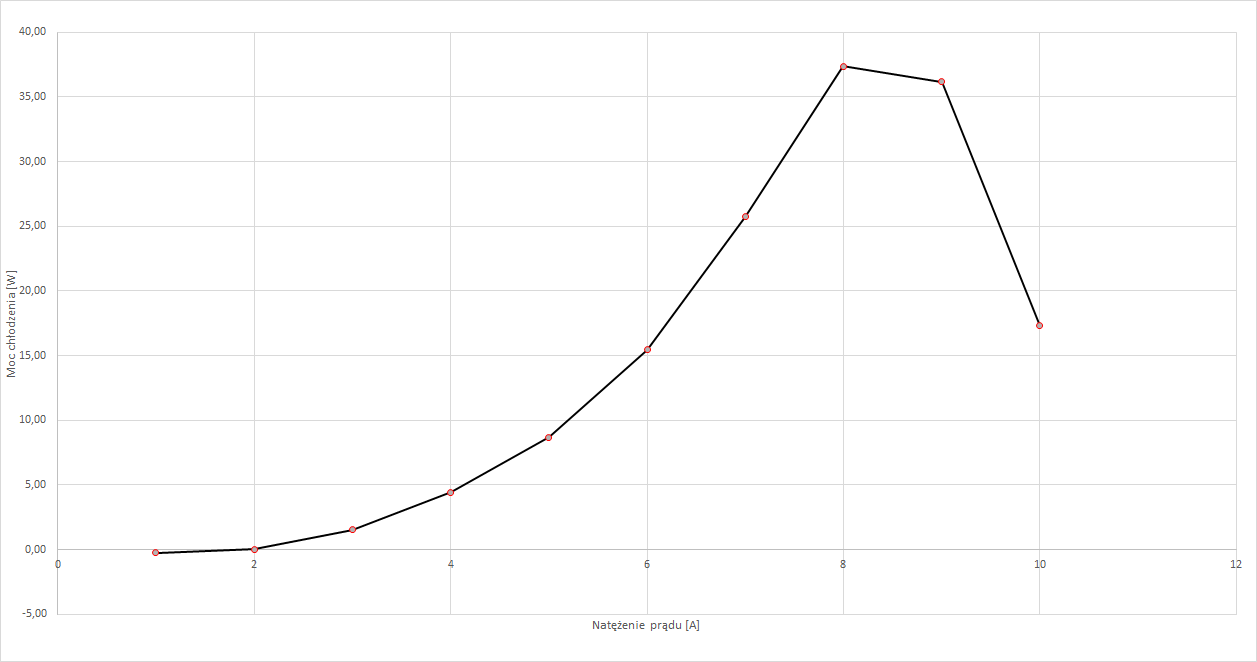
\includegraphics[width=\textwidth]{Qc_wykres.png}
    \caption{Sprawności modułu Peltiera jako pompy ciepła od natężenia prądu}
    \end{figure}
\end{center}

Na podstawie wykresu można wywnioskować ,że największą moc chłodzenia dla badanego układu moduł Peltiera generuje gdy podane zostanie na niego natężenie prądu równe w przybliżeniu 8A. Co za tym idzie przy ustalonym napięciu 15V i natężeniu 8A moduł osiąga największą efektywność generując tym samym w chwili czasu t = 180s moc 108 Wat. Obliczona wartość mocy chłodzenia($Q_c$) została wykorzystana w następnym rozdziale dotyczącym regulacji zbudowanego układu. Wartość natężenia prądu wynosząca 8 amper została ustawiona jako 100\% mocy wzmacniacza modułu Peltiera. 
\chapter{Regulacja układu}
W zbudownym układzie zastosowano dwa rodzaje regulacji które zostały zaprogramowane w programie LOGO!SoftComfort opisanym w rozdziale czwartym. Poniższa cześć pracy opisuje program oraz kolejno regulacje dwupołożeniową, regulację przy pomocy regulatora PI oraz reakcję poszczególnych regulatorów na dodawanie do układu zakłóceń. W części poświęconej regulatorowi PI oprócz opisu regulacji zawarto informacje na temat sposobu doboru nastaw regulatora oraz opis wybranej metody wraz z jej uzasadnieniem.

Zbadano również jak układ reaguje na zakłócenia w postaci wydzielanego ciepła przez zastosowane rezystory. Badania przeprowadzono dla dwóch typów regulatorów. Po wykonaniu badań porównano dwie metody regulacji w zakresach szybkości i dokładności w osiąganiu wartości zadanej temperatury. 
\section{Regulator dwupołożeniowy}
Regulacja dwupołożeniowa polega na cyklicznym załączaniu i wyłączaniu pełnej mocy urządzenia tak aby utrzymywana była temperatura zadana. Takie układy z regulacji stosowane są w obiektach które nie wymagają dokładnego utrzymywania zadanej wartości i dopuszczają oscylacje. Regulatory dwupołożeniowe dzięki swojej prostej budowie oraz niezawodności w działaniu znalazły szerokie zastosowanie w wielu powszechnie stosowanych układach regulacji. Praktycznymi przykładami urządzeń wykorzystujących regulację dwupołożeniową są między innymi lodówka i żelazko.
\subsection{Opis regulacji}
W projekcie został zastosowany regulator dwupołożeniowy pozwalający na regulowanie temperatury w komorze chłodniczej. Na zastosowany w układzie moduł Peltiera podawane natężenie prądu zgodnie z poniższym wzorem:
\begin{center}
\begin{equation*}
    I(t) = \left\{ \begin{array}{ll}
    8A & \textrm{gdy $E \geq SP$}\\
    0A & \textrm{gdy $E < SP$}\\
\end{array} \right.
\end{equation*}
\end{center}
gdzie: \\
E - wartość zmierzona przez czujnik temperatury, \\
SP - zadana temperatura. \\

Przebieg zmiany temperatury w czasie w komorze termicznej przy wykorzystaniu do kontroli temperatury regulatora dwupołorzeniowego został przedstawiony na rysunku

\section{Regulator typu PI}
Regulacja typu PI jest odmianą klasycznego sterowania PID wykorzystującą wyłącznie człon proporcjonalny i całkujący regulatora PID do kontroli regulowanego układu. W praktyce do regulacji układów wolnozmiennych najczęściej używa się regulatorów typu PI z uwagi na wolne zmiany regulowanych wartości. Wartość wyjściowa czujnika temperatury jest wprowadzana do bloczka regulatora jako zmienna wejściowa[22]:
\begin{equation*}
    \begin{array}{c}
        e(t) = SP - PV \\ \\
        u(t) = K_{p}e(t) + \frac{K_p}{T_i} \int_{0}^t e(t)dt \\ \\
    \end{array}
\end{equation*}
Dwie wartości będące nastawami regulatora PI to wzmocnienie $K_p$ i stała czasu całkowania $Ti$. $K_p$ stanowi wzmocnienie błędu proporcjonalnego i członu całkującego. Zwiększenie wartości wzmocnienia powoduje bardziej dynamiczną reakcję na błędy pomiarowe oddalone od temperatury zadanej. Wartość SP jest wartością zadaną natomiast zmienna PV jest wartością zmierzoną przez czujnik temperatury która może odbiegać od wartości zadanej. Błąd wartości zadanej e(t) jest różnicą między SP i PV i definiuje się go jako $e(t) = SP-PV$[22].
\subsection{Dobór nastaw regulatora}
W celu doboru nastaw regulatora wykorzystano pierwszą metodę Zieglera- Nicholsa. Wybrano tą metodę ponieważ nie wymaga ona dokładnej znajomości regulowanego obiektu. Wykorzystana metoda polega na aproksymacji parametrów regulatora wykorzystując odpowiedź układu na pobudzenie skokowe. Odpowiedź badanego obiektu na pobudzenie skokowe wynoszące 3A została przedstawiona graficznie na rysunku 6.1.
\begin{center}
\begin{figure}[h!]
    \centering
    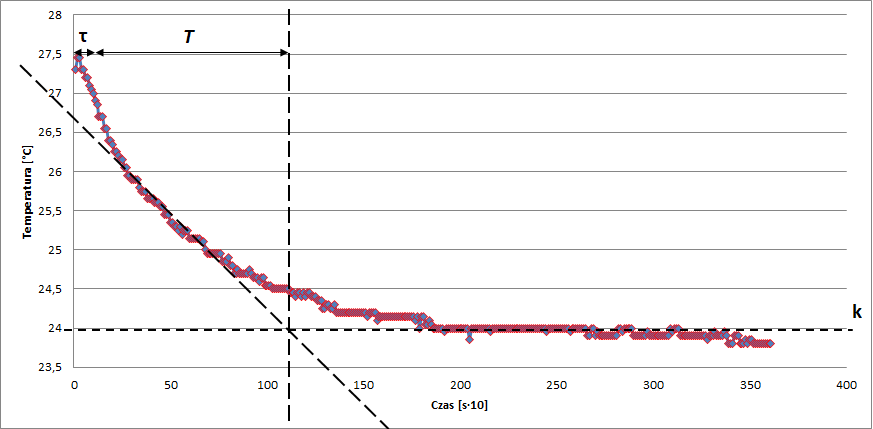
\includegraphics[width=\textwidth]{Odpowiedz_skokowa_regulacja.png}
    \caption{Odpowiedź skokowa układu na pobudzenie 3A}
    \end{figure}
\end{center}

Odpowiedź układu została aproksymowana charakterystyką skokową pierwszego rzędu co pozwala na odczytanie dwóch wartości charakterystycznych dla układu[18]:\\
$\tau$ - opóźnienie reakcji układu na pobudzenie. \\
$T$ - stała czasowa, styczna do przebiegu odpowiedzi skokowej w punkcie przegięcia.\\

Sposób wyznaczenia parametrów regulatora pierwszą metodą Zieglera-Nicholsa na podstawie wartości odczytanych z rysunku 6.1 przedstawia tabela 6.2.

\begin{table}[h!]
\begin{tabularx}{\textwidth}{|c|c|c|}
\hline
\rowcolor{lightgray}
Rodzaj regulacji & Kp & Ti \\ \hline
\multirow{2}{*}{Przeregulowanie = 0\%,  Minimum czasu reg. $t_r$ } & \multirow{2}{*}{$0,6 \cdot \frac{T}{\tau}$} & \multirow{2}{*}{$0,8\tau + 0,5T$} \\
 & &\\\hline
\multirow{2}{*}{Przeregulowanie = 20\%,  Minimum czasu reg. $t_r$ } & \multirow{2}{*}{$0,7 \cdot \frac{T}{\tau}$} & \multirow{2}{*}{$\tau + 0,3T$} \\
 & &\\ \hline
\multirow{2}{*}{$\min \int_{0}^{\infty}e^{2}(t)dt$} & \multirow{2}{*}{$\frac{T}{\tau}$} & \multirow{2}{*}{$\tau + 0,35T$} \\
 & &\\ \hline
\end{tabularx}
   \caption{Nastawy dla regulatora PI}
\end{table}

Wykorzystując wzory zawarte w tabeli 6.2 oraz wyznaczone charakterystyczne wartości $\tau = 50$ oraz $T = 1100$ obliczono parametry nastaw dla trzech różnych sposobów regulacji.

\subsubsection{Regulacja z zerowym przeregulowaniem}
    \begin{equation*}
    \begin{array}{c}
     \tau = 50, T = 1100 \\ \\
    K_{p} = 0,6 \cdot \frac{T}{\tau} = 0,6 \cdot \frac{1100}{50} = 13,2 \\ \\
    T_{i} = 0,8\tau + 0,5T = 0,8 \cdot 50 + 0,5 \cdot 1100 = 590[s]\\ \\
    \end{array}
    \end{equation*}
    Zastosowanie obliczonych nastaw pozwala na uzyskanie aperiodycznej odpowiedzi układu minimalizując tym samym czas regulacji.
\subsubsection{Regulacja z przeregulowaniem wynoszącym 20\%}
    \begin{equation*}
    \begin{array}{c}
     \tau = 50, T = 1100 \\ \\
    K_{p} = 0,7 \cdot \frac{T}{\tau} = 0,7 \cdot \frac{1100}{50} = 15,4 \\ \\
    T_{i} = \tau + 0,3T = 50 + 0,3 \cdot 1100 = 380[s]\\ \\
    \end{array}
    \end{equation*}
    Zastosowanie obliczonych nastaw generuje odpowiedź układu z oscylacjami o przeregulowaniu wynoszącym 20\% oraz minimalnym czasie regulacji.
\subsubsection{Odpowiedź minimalizująca całkę ISE}
    \begin{equation*}
    \begin{array}{c}
     \tau = 50, T = 1100 \\ \\
    K_{p} = \frac{T}{\tau} = \frac{1100}{50} = 22 \\ \\
    T_{i} = \tau + 0,35T = 50 + 0,35 \cdot 1100 = 435[s]\\ \\
    \end{array}
    \end{equation*}
    Zastosowanie obliczonych w ten sposób nastaw pozwala zminimalizować całki kwadratu uchybu.


\subsection{Regulacja na podstawie obliczonych nastaw}
Obliczone w części 6.2.1 nastawy zostały zaimplementowane w programie. Dla każdej obliczonej pary nastaw wykonano badania czasu regulacji i wielkości przeregulowań. Wszystkie badania zostały wykonane dla takiej samej temperatury początkowej wynoszącej 27,75\textdegree{}C. Temperatura docelowa którą układ miał osiągnąć ustawiono na 25,00\textdegree{}C. Pomiary temperatury zostały wykonane przy pomocy czujnika zamieszczonego wewnątrz komory termicznej i zbierane do bazy danych przy pomocy narzędzia LOO!AccessTool opisanego w rozdziale czwartym.

\subsubsection{Regulacja z zerowym przeregulowaniem}
Na rysunku 6.2 został przedstawiony przebieg temperatury w komorze chłodniczej w czasie. Układ dochodzi do ustawionej temperatury bez przeregulowań w czasie około 25 minut. Na rysunku można również zauważyć wiele pomiarów nieznacznie oddalonych od poprawnego przebiegu regulacji. Są one spowodowane niedokładnością pomiarową zastosowanych urządzeń oraz wpływem warunków zewnętrznych na komorę termiczną.

\begin{center}
\begin{figure}[h!]
    \centering
    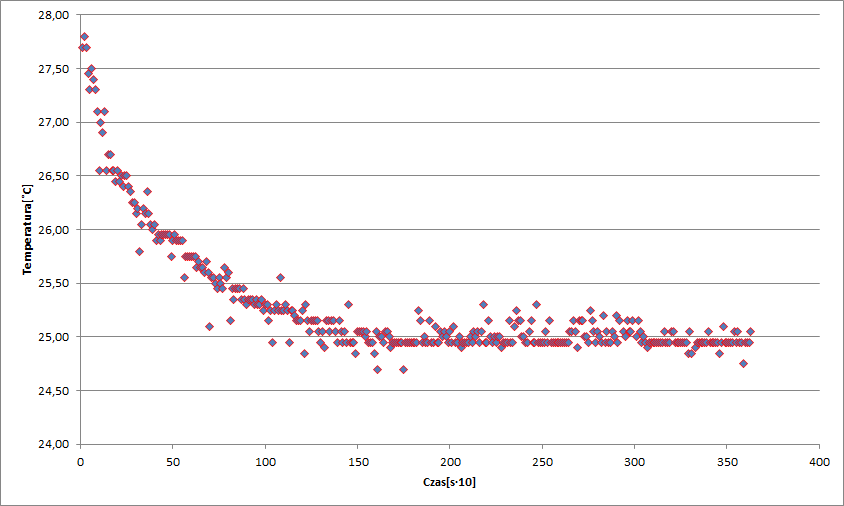
\includegraphics[width=\textwidth]{ZN11.png}
    \caption{Przebieg temperatury w komorze chłodniczej dla Kp = 13,2 i Ti = 590s}
    \end{figure}
\end{center}

\subsubsection{Regulacja z przeregulowaniem 20\%}
Rysunek 6.3 przedstawia regulacje z przeregulowaniem. Na podstawie przebiegu temperatury w czasie można wywnioskować, że układ dąży do zadanej temperatury wynoszącej 25,00\textdegree{}C jednak po jej osiągnięciu ją przekracza o około 0,25\textdegree{}C. Wartość ta stanowi przeregulowanie będące stanowiące 20\% różnicy temperatur pomiędzy wartością początkową a zadaną. Przez zaistniałe przeregulowanie czas regulacji układu wydłużył się do około 30 minut.
\begin{center}
\begin{figure}[h!]
    \centering
    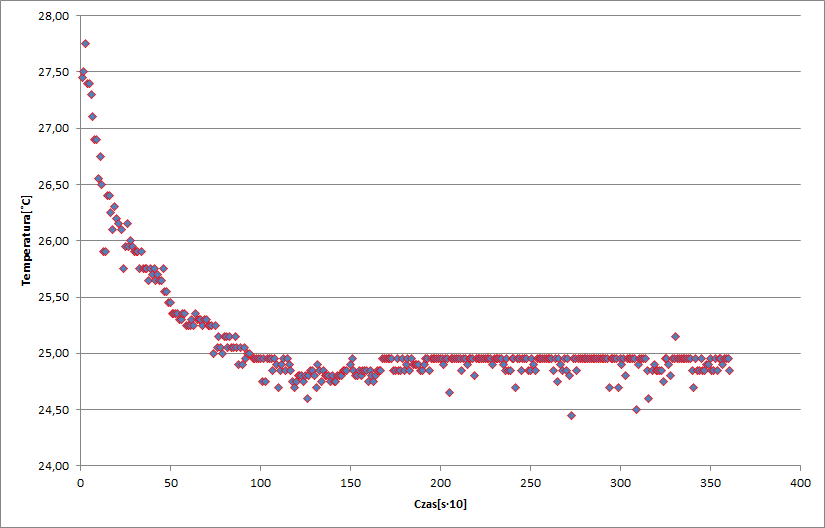
\includegraphics[width=\textwidth]{ZN12.png}
    \caption{Przebieg temperatury w komorze chłodniczej dla Kp = 15,4 i Ti = ,380s}
    \end{figure}
\end{center}

\subsubsection{Regulacja z minimalną całką kwadratu uchybu regulacji}
Na podstawie nastaw obliczonych tak aby zminimalizować błąd kwadratu całki uchybu regulacji został wygenerowany rysunek 6.4. Całka kwadratu uchybu regulacji (ISE) jest miarą wydajności systemu. Im mniejsza całka kwadratu błędu systemu w przedziale czasu tym regulator jest dokładniejszy. Na podstawie otrzymanego przebiegu można zauważyć ,że układ najszybciej zmierza do wartości zadanej. Spowodowane jest to dość dużym wzmocnieniem Kp wynoszącym 22 oraz krótkim czasem Ti. Po 35 minutach badania układu pojawiają się szumy spowodowane niedokładną izolacją całego układu i zakłuceniami losowymi. Z racji dużego wzmocnienia układ reaguje na błędne pomiary gwałtownymi zmianami mocy na ogniwie Peltiera co skutkuje dużym rozrzutem mierzonych wartości po 35 minucie badania. 

\begin{center}
\begin{figure}[h!]
    \centering
    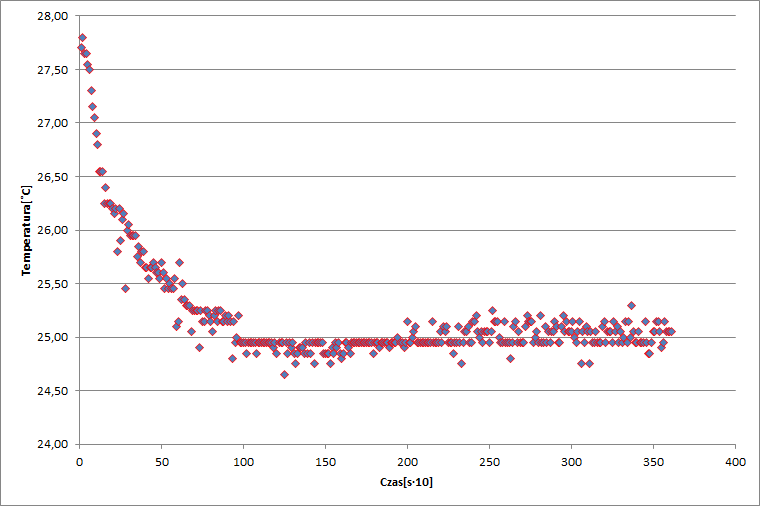
\includegraphics[width=\textwidth]{ZN13.png}
    \caption{Przebieg temperatury w komorze chłodniczej dla Kp = 22 i Ti = ,435s}
    \end{figure}
\end{center}

\section{Dodanie zakłóceń do układu regulacji}
W celu wprowadzenia do badanego układu zakłóceń zostały wprowadzone rezystory wysokich mocy. Rezystory pełnią funkcję źródła ciepła i powodują nagrzewanie się komory termicznej. Aby sprawdzić działanie regulatorów w trakcie wystąpienia zakłóceń w momencie ustabilizowania się układu regulacji włączono źródło ciepła na 100\% mocy na czas pięciu minut. Na podstawie zebranych danych pomiarowych z czujnika temperatury wewnątrz komory termicznej wykreślono przebiegi temperatury w czasie dla regulatora dwupołożeniowego oraz regulatora PI które dają w przybliżeniu zerowe przeregulowanie i minimalny czas regulacji. Na podstawie zebranych danych porównano uchyby regulacji spowodowane włączeniem źródła ciepła jak i czas powrotu do zadanej temperatury po wyłączeniu rezystorów.

Wyniki przeprowadzonych badań zostały przedstawione na poniższych rysunkach.
\section{Porównanie sposobów regulacji}

\chapter{Podsumowanie}
W pracy zostały zrealizowane wszystkie założenia projektowe. Została przytoczona część teoretyczna pozwalająca na zrozumienie reakcji zachodzących w termoelemencie w momencie przepływu przez niego prądu elektrycznego. Zostały omówione podstawowe prawa i efekty termoelektryczne takie jak efekt Seebecka, efekt Thomsona, zjawisko Joul'a na efekcie Peltiera będącym tematem niniejszej pracy kończąc.

Przedstawiony został kompletny schemat budowy urządzenia pozwalającego na pomiar i badanie zmian zachodzących na module Peltiera wraz z możliwością jego regulacji. Rozdział trzeci pracy zawiera szczegółowe informacje na temat wykorzystanych w projekcie elementów jak i ich opis.

Z wykorzystaniem programu LOGO!SoftComfort oraz narzędzia  LOGO!AccessTool opisanych w rozdziale czwartym wykonano badania zastosowanego ogniwa Peltiera typu TEC1-12715. Zmierzono temperatury bloków aluminiowych umieszczonych bezpośrednio nad i pod modułem termoelektrycznym i na ich podstawie obliczono takie wartości jak moc chłodzenia i moc grzania w zależności od podawanego na moduł natężenia prądu.

Na podstawie dokonanych badań i ustalonego natężenia prądu dla którego moc chłodzenia ogniwem jest największa przeprowadzono regulację temperatury w zbudowanej komorze termicznej. Zbadane zostały dwa typy regulatorów regulator dwupołożeniowy oraz regulator PI. Aby sprawdzić jakość użytych regulatorów przeprowadzono próby szybkości regulacji wprowadzając do układu odpowiednie zakłócenia.


\addcontentsline{toc}{chapter}{\bibname}
\begin{thebibliography} 
\\
\bibitem{Filin},,Termoelektryczne urządzenia chłodnicze’’, Sergiey Filin
\bibitem{KK}https://elportal.pl/pdf/k01/20\_05.pdf
\bibitem{LOGO}https://www.automatyka.siemens.pl/docs/docs\_ia/Podrecznik\_Siemens\_LOGO8\_PL.pdf
\bibitem{Zadajnik}http://anleitung.joy-it.net/wp-content/uploads/2018/09/JT-DPS5015-Manual-1.pdf
\bibitem{LOGO!}Siemens LOGO! Manual, 11/2017 [numer: A5E33039675 - AE]
\bibitem{PT-10}https://www.telmatik.pl
\bibitem{PPT}http://lpf.wppt.pwr.edu.pl/opisy/cw038b.pdf
\bibitem{Went-z}https://sklep.eltron.pl/pl/p/18182546394022/ee92252b1-a99
\bibitem{Went-c}https://sklep.eltron.pl/pl/p/184750184159/eec0252b3-a99
\bibitem{Rezystory}www.aksotronik.com.pl
\bibitem{Wylacznik}https://pl.traconelectric.com
\bibitem{Przekazniki}https://www.relpol.pl/Produkty/Przekazniki-Miniaturowe
\bibitem{Ogniwo}http://www.thermonamic.com/TEC1-12715-English.PDF
\bibitem{Radiator}https://www.silentiumpc.com/pl/product/fera-3-he1224/
\bibitem{Wzmacniacz-mocy}https://archiwum.allegro.pl/oferta/regulator-obrotow-silnika-pwm-softstart-12v-20a-n3-i6957413878.html
\bibitem{Badania1ang}https://pdfs.semanticscholar.org/ccce/7badad4f0421a52373aa94e496f3e6291abd.pdf
\bibitem{Badania2Pwr}http://lpf.wppt.pwr.edu.pl/opisy/cw038b.pdf
\bibitem{PI-regulacja}https://automatykab2b.pl/technika/46618-strojenie-pid-metody-doboru-nastaw-czesc-1
\bibitem{ZN}https://en.wikipedia.org/wiki/Ziegler\%E2\%80\%93Nichols\_method\#cite\_note-1
\bibitem{ZN1}http://educypedia.karadimov.info/library/Ziegler\_Nichols.pdf
\bibitem{ZNTabela}https://eia.pg.edu.pl/documents/184139/35251635/PA\_CW\_T13\_T14\_Pomoc.pdf
\bibitem{PI-opis}https://apmonitor.com/pdc/index.php/Main/ProportionalIntegralControl
\end{thebibliography}

\listoffigures
\addcontentsline{toc}{chapter}{Spis rysunków}
\listoftables
\addcontentsline{toc}{chapter}{Spis tabel}
\chapter*{Spis załączników}
\addcontentsline{toc}{chapter}{Spis załączników}
\begin{enumerate}
    \item Lista sygnałów
    \item Spis schematów elektrycznych i ideowych
    \item Schematy elektryczne
\end{enumerate}
\end{document}